\documentclass[acmsmall,screen]{acmart}

%%
%% \BibTeX command to typeset BibTeX logo in the docs
\AtBeginDocument{%
  \providecommand\BibTeX{{%
    Bib\TeX}}}

% %% Rights management information.  This information is sent to you
% %% when you complete the rights form.  These commands have SAMPLE
% %% values in them; it is your responsibility as an author to replace
% %% the commands and values with those provided to you when you
% %% complete the rights form.
% \setcopyright{acmlicensed}
% \copyrightyear{2018}
% \acmYear{2018}
% \acmDOI{XXXXXXX.XXXXXXX}

% %% These commands are for a PROCEEDINGS abstract or paper.
% \acmConference[Conference acronym 'XX]{Make sure to enter the correct
%   conference title from your rights confirmation email}{June 03--05,
%   2018}{Woodstock, NY}
% %%
%%  Uncomment \acmBooktitle if the title of the proceedings is different
%%  from ``Proceedings of ...''!
%%
%%\acmBooktitle{Woodstock '18: ACM Symposium on Neural Gaze Detection,
%%  June 03--05, 2018, Woodstock, NY}
% \acmISBN{978-1-4503-XXXX-X/18/06}


%%
%% Submission ID.
%% Use this when submitting an article to a sponsored event. You'll
%% receive a unique submission ID from the organizers
%% of the event, and this ID should be used as the parameter to this command.
% \acmSubmissionID{136}

%%
%% For managing citations, it is recommended to use bibliography
%% files in BibTeX format.
%%
%% You can then either use BibTeX with the ACM-Reference-Format style,
%% or BibLaTeX with the acmnumeric or acmauthoryear sytles, that include
%% support for advanced citation of software artefact from the
%% biblatex-software package, also separately available on CTAN.
%%
%% Look at the sample-*-biblatex.tex files for templates showcasing
%% the biblatex styles.
%%

%%
%% The majority of ACM publications use numbered citations and
%% references.  The command \citestyle{authoryear} switches to the
%% "author year" style.
%%
%% If you are preparing content for an event
%% sponsored by ACM SIGGRAPH, you must use the "author year" style of
%% citations and references.
%% Uncommenting
%% the next command will enable that style.
% \citestyle{acmauthoryear}
\citestyle{acmnumeric}


\usepackage[T1]{fontenc}

\usepackage{tikz}
\usetikzlibrary{automata,arrows,positioning}
\usepackage{multirow}
\usepackage{subfigure}
\usepackage{makecell}
\usepackage{algorithmic}
\usepackage{xcolor,xspace}
\usepackage{mathtools}
\usepackage{colortbl}
\usepackage{enumitem}
\usepackage{hhline}
\usepackage{textcomp}
\usepackage{xcolor}
\usepackage{booktabs}
\usepackage{hyperref}
\usepackage{graphicx}
\usepackage{relsize}
\usepackage{makecell}
\usepackage{wrapfig}
\usepackage{bbding}
\usepackage{algorithmic}
% \usepackage{adjustbox}
% \usepackage{multicol}

% \usepackage{amsmath, amssymb, amsfonts}
\usepackage[algoruled,noend,linesnumbered]{algorithm2e}%

%
\definecolor{mygray}{gray}{.85}
\newcommand{\yd}[1]{\textcolor{blue}{#1}}
% \newcommand{\lei}[1]{\textcolor{cyan}{#1}}

% \newcommand{\minor}[1]{\textcolor{blue}{{#1}}}
% \newcommand{\major}[1]{\textcolor{red}{{#1}}}

\newcommand{\minor}[1]{\textcolor{black}{{#1}}}
\newcommand{\major}[1]{\textcolor{black}{{#1}}}

% \newcommand{\red}[1]{\textcolor{red}{#1}}
\newcommand{\tool}{{\sf BFAVerifier}\xspace}
\newcommand{\ReTool}{{\sf Quadapter$^\ast$}\xspace}

\newcommand{\clever}{{\sf CLEVER}\xpace}
\newcommand{\deepPoly}{{\sf DeepPoly}\xspace}
% \newcommand{\deepPolyR}{{\sf DeepPolyR}\xspace}
\newcommand{\symPoly}{{\sf SymPoly}\xspace}
\newcommand{\mR}{{\mathcal{R}}}
\newcommand{\mI}{{\mathcal{I}}}
\newcommand{\mO}{{\mathcal{O}}}
\newcommand{\mP}{{\mathcal{P}}}
\newcommand{\mT}{{\mathcal{T}}}
\newcommand{\mB}{{\mathcal{B}}}
\newcommand{\mA}{{\mathcal{A}}}
\newcommand{\mN}{{\mathcal{N}}}
\newcommand{\bs}[1]{{\mathbf{#1}}}
\newcommand{\act}{{\textrm{act}}}
\newcommand{\aff}{{\textrm{aff}}}
\newcommand{\slb}{{\le}}
\newcommand{\sub}{{\ge}}
\newcommand{\mm}{\mathfrak{m}}
\newcommand{\kk}{\mathfrak{k}}

\newcommand{\Continue}{{\bf continue}}
\newcommand{\nn}{\mathfrak{n}}
\newcommand{\VanillaVerifier}{{\sf VanillaVerifier}\xspace}
\usepackage{booktabs}
\usepackage{multirow}
\newcommand{\tabincell}[2]{\begin{tabular}{@{}#1@{}}#2\end{tabular}}


\makeatletter
\newcommand{\Rmnum}[1]{\expandafter\@slowromancap\romannumeral #1@}
\makeatother

%%
%% end of the preamble, start of the body of the document source.
\begin{document}


%%
%% The "title" command has an optional parameter,
%% allowing the author to define a "short title" to be used in page headers.
\title{Verification of Bit-Flip Attacks against Quantized Neural Networks}

% %%
% %% The "author" command and its associated commands are used to define
% %% the authors and their affiliations.
% %% Of note is the shared affiliation of the first two authors, and the
% %% "authornote" and "authornotemark" commands
% %% used to denote shared contribution to the research.
%\author{Ben Trovato}
%\authornote{Corresponding author.}
%\email{trovato@corporation.com}
% \orcid{1234-5678-9012}
% \author{G.K.M. Tobin}
% \authornotemark[1]
% \email{webmaster@marysville-ohio.com}
%\affiliation{%
%  \institution{Institute for Clarity in Documentation}
%  \city{Dublin}
%  \state{Ohio}
%  \country{USA}
%}

\author{Yedi Zhang}
\affiliation{%
  \institution{National University of Singapore}
  \city{Singapore}
  \country{Singapore}}
  \email{yd.zhang@nus.edu.sg}


 \author{Lei Huang}
 \affiliation{%
   \institution{ShanghaiTech University}
   \city{Shanghai}
   \country{China}}
   \email{huanglei@shanghaitech.edu.cn}

 \author{Pengfei Gao}
 \affiliation{%
  \institution{ByteDance Inc}
  \city{Beijing}
  \country{China}}
   \email{gaopengfei.se@bytedance.com}

 \author{Fu Song}
 \authornote{Corresponding author.}
 \affiliation{%
   \institution{Key Laboratory of System Software (Chinese Academy of Sciences) and State Key Laboratory of Computer Science, Institute of Software, Chinese Academy of Sciences}
   \city{Beijing}
   \country{China}}
\additionalaffiliation{
\institution{University of Chinese Academy of Sciences}
  \city{Beijing}
  \country{China}}
\additionalaffiliation{
\institution{Nanjing Institute of Software Technology}
  \city{Nanjing}
  \country{China}}
\email{songfu@ios.ac.cn}
   
\author{Jun Sun}
\affiliation{%
  \institution{Singapore Management University}
  \city{Singapore}
  \country{Singapore}}
\email{junsun@smu.edu.sg}

\author{Jin Song Dong}
\affiliation{%
  \institution{National University of Singapore}
  \city{Singapore}
  \country{Singapore}}
\email{dcsdjs@nus.edu.sg}

% \author{John Smith}
% \affiliation{%
%   \institution{The Th{\o}rv{\"a}ld Group}
%   \city{Hekla}
%   \country{Iceland}}
% \email{jsmith@affiliation.org}

% \author{Julius P. Kumquat}
% \affiliation{%
%   \institution{The Kumquat Consortium}
%   \city{New York}
%   \country{USA}}
% \email{jpkumquat@consortium.net}

%%
%% By default, the full list of authors will be used in the page
%% headers. Often, this list is too long, and will overlap
%% other information printed in the page headers. This command allows
%% the author to define a more concise list
%% of authors' names for this purpose.
 \renewcommand{\shortauthors}{Zhang et al.}

%%
%% The abstract is a short summary of the work to be presented in the
%% article.
\begin{abstract}
  In the rapidly evolving landscape of neural network security, the resilience of neural networks against bit-flip attacks (i.e., an attacker maliciously flips an extremely small amount of bits within its parameter storage memory system to induce harmful behavior), has emerged as a relevant area of research. Existing studies suggest that quantization may serve as a viable defense against such attacks. Recognizing the documented susceptibility of real-valued neural networks to such attacks and the comparative robustness of quantized neural networks (QNNs), in this work, we introduce \tool, the first verification framework designed to formally verify the absence of bit-flip attacks or to identify all vulnerable parameters in a sound and rigorous manner.
\tool comprises two integral components: an abstraction-based method and an MILP-based method.
Specifically, we first conduct a reachability analysis with respect to symbolic parameters that represent the potential bit-flip attacks, based on a novel abstract domain with a sound guarantee. If the reachability analysis fails to prove the resilience of such attacks, then we encode this verification problem into an equivalent MILP problem which can be solved by off-the-shelf solvers. 
Therefore, \tool is sound, complete, and reasonably efficient. We conduct extensive experiments, which demonstrate its effectiveness and efficiency across various network architectures, quantization bit-widths, and adversary capabilities. 
%The source code of our tool and benchmarks are available at \url{https://anonymous.4open.science/r/BFAVerifier-B315}.
\end{abstract}

%%
%% The code below is generated by the tool at http://dl.acm.org/ccs.cfm.
%% Please copy and paste the code instead of the example below.
%%
\begin{CCSXML}
  <ccs2012>
     <concept>
         <concept_id>10010147.10010257.10010293.10010294</concept_id>
         <concept_desc>Computing methodologies~Neural networks</concept_desc>
         <concept_significance>500</concept_significance>
      </concept>
    
    <concept>
        <concept_id>10011007.10011074.10011099.10011692</concept_id>
         <concept_desc>Software and its engineering~Formal software verification</concept_desc>
         <concept_significance>500</concept_significance>
     </concept>
    
 %   <concept>
 %        <concept_id>10002978.10002986.10002990</concept_id>
 %        <concept_desc>Security and privacy~Logic and verification</concept_desc>
 %        <concept_significance>500</concept_significance>
  %   </concept>
   
   <concept>
        <concept_desc>Security and privacy~Software security engineering</concept_desc>
       <concept_significance>500</concept_significance>
    </concept>
  </ccs2012>

\end{CCSXML}

\ccsdesc[500]{Computing methodologies~Neural networks}
\ccsdesc[500]{Software and its engineering~Formal software verification}
%\ccsdesc[500]{Security and privacy~Logic and verification}
\ccsdesc[500]{Security and privacy~Software security engineering}

%%
%% Keywords. The author(s) should pick words that accurately describe
%% the work being presented. Separate the keywords with commas.
\keywords{Bit-Flip Attacks, Quantized Neural Networks, Formal Verification, Robustness}
% %% A "teaser" image appears between the author and affiliation
% %% information and the body of the document, and typically spans the
% %% page.
% \begin{teaserfigure}
%   \includegraphics[width=\textwidth]{sampleteaser}
%   \caption{Seattle Mariners at Spring Training, 2010.}
%   \Description{Enjoying the baseball game from the third-base
%   seats. Ichiro Suzuki preparing to bat.}
%   \label{fig:teaser}
% \end{teaserfigure}

% \received{20 February 2007}
% \received[revised]{12 March 2009}
% \received[accepted]{5 June 2009}

%%
%% This command processes the author and affiliation and title
%% information and builds the first part of the formatted document.
\maketitle


\section{Introduction}


\begin{figure}[t]
\centering
\includegraphics[width=0.6\columnwidth]{figures/evaluation_desiderata_V5.pdf}
\vspace{-0.5cm}
\caption{\systemName is a platform for conducting realistic evaluations of code LLMs, collecting human preferences of coding models with real users, real tasks, and in realistic environments, aimed at addressing the limitations of existing evaluations.
}
\label{fig:motivation}
\end{figure}

\begin{figure*}[t]
\centering
\includegraphics[width=\textwidth]{figures/system_design_v2.png}
\caption{We introduce \systemName, a VSCode extension to collect human preferences of code directly in a developer's IDE. \systemName enables developers to use code completions from various models. The system comprises a) the interface in the user's IDE which presents paired completions to users (left), b) a sampling strategy that picks model pairs to reduce latency (right, top), and c) a prompting scheme that allows diverse LLMs to perform code completions with high fidelity.
Users can select between the top completion (green box) using \texttt{tab} or the bottom completion (blue box) using \texttt{shift+tab}.}
\label{fig:overview}
\end{figure*}

As model capabilities improve, large language models (LLMs) are increasingly integrated into user environments and workflows.
For example, software developers code with AI in integrated developer environments (IDEs)~\citep{peng2023impact}, doctors rely on notes generated through ambient listening~\citep{oberst2024science}, and lawyers consider case evidence identified by electronic discovery systems~\citep{yang2024beyond}.
Increasing deployment of models in productivity tools demands evaluation that more closely reflects real-world circumstances~\citep{hutchinson2022evaluation, saxon2024benchmarks, kapoor2024ai}.
While newer benchmarks and live platforms incorporate human feedback to capture real-world usage, they almost exclusively focus on evaluating LLMs in chat conversations~\citep{zheng2023judging,dubois2023alpacafarm,chiang2024chatbot, kirk2024the}.
Model evaluation must move beyond chat-based interactions and into specialized user environments.



 

In this work, we focus on evaluating LLM-based coding assistants. 
Despite the popularity of these tools---millions of developers use Github Copilot~\citep{Copilot}---existing
evaluations of the coding capabilities of new models exhibit multiple limitations (Figure~\ref{fig:motivation}, bottom).
Traditional ML benchmarks evaluate LLM capabilities by measuring how well a model can complete static, interview-style coding tasks~\citep{chen2021evaluating,austin2021program,jain2024livecodebench, white2024livebench} and lack \emph{real users}. 
User studies recruit real users to evaluate the effectiveness of LLMs as coding assistants, but are often limited to simple programming tasks as opposed to \emph{real tasks}~\citep{vaithilingam2022expectation,ross2023programmer, mozannar2024realhumaneval}.
Recent efforts to collect human feedback such as Chatbot Arena~\citep{chiang2024chatbot} are still removed from a \emph{realistic environment}, resulting in users and data that deviate from typical software development processes.
We introduce \systemName to address these limitations (Figure~\ref{fig:motivation}, top), and we describe our three main contributions below.


\textbf{We deploy \systemName in-the-wild to collect human preferences on code.} 
\systemName is a Visual Studio Code extension, collecting preferences directly in a developer's IDE within their actual workflow (Figure~\ref{fig:overview}).
\systemName provides developers with code completions, akin to the type of support provided by Github Copilot~\citep{Copilot}. 
Over the past 3 months, \systemName has served over~\completions suggestions from 10 state-of-the-art LLMs, 
gathering \sampleCount~votes from \userCount~users.
To collect user preferences,
\systemName presents a novel interface that shows users paired code completions from two different LLMs, which are determined based on a sampling strategy that aims to 
mitigate latency while preserving coverage across model comparisons.
Additionally, we devise a prompting scheme that allows a diverse set of models to perform code completions with high fidelity.
See Section~\ref{sec:system} and Section~\ref{sec:deployment} for details about system design and deployment respectively.



\textbf{We construct a leaderboard of user preferences and find notable differences from existing static benchmarks and human preference leaderboards.}
In general, we observe that smaller models seem to overperform in static benchmarks compared to our leaderboard, while performance among larger models is mixed (Section~\ref{sec:leaderboard_calculation}).
We attribute these differences to the fact that \systemName is exposed to users and tasks that differ drastically from code evaluations in the past. 
Our data spans 103 programming languages and 24 natural languages as well as a variety of real-world applications and code structures, while static benchmarks tend to focus on a specific programming and natural language and task (e.g. coding competition problems).
Additionally, while all of \systemName interactions contain code contexts and the majority involve infilling tasks, a much smaller fraction of Chatbot Arena's coding tasks contain code context, with infilling tasks appearing even more rarely. 
We analyze our data in depth in Section~\ref{subsec:comparison}.



\textbf{We derive new insights into user preferences of code by analyzing \systemName's diverse and distinct data distribution.}
We compare user preferences across different stratifications of input data (e.g., common versus rare languages) and observe which affect observed preferences most (Section~\ref{sec:analysis}).
For example, while user preferences stay relatively consistent across various programming languages, they differ drastically between different task categories (e.g. frontend/backend versus algorithm design).
We also observe variations in user preference due to different features related to code structure 
(e.g., context length and completion patterns).
We open-source \systemName and release a curated subset of code contexts.
Altogether, our results highlight the necessity of model evaluation in realistic and domain-specific settings.






\section{Preliminary}
\label{sec:3}
% 在本节,我们将分别定义实现高效CBE的三个要素:accuracy,convergence, scalability,并分析影响它们的要素。
In this section, we start by symbolically introducing the working process of CBE. Afterwards, we introduce the key objectives for achieving efficient CBE: accuracy, convergence, and scalability, and analyze the factors that influence them.
We mainly discuss the pair-wise evaluation scenario (where the judge provides preference between two models per time) for its wide applications \citep{paireval,allpair}. Actually, list-wise preferences can be easily converted into pair-wise ones, as demonstrated in \S\ref{sec:5.4-2}, so the discussions below are general for CBE.
% 考虑到pair-wise comparison(Judge每次给出对两个models的preference)是CBE的最典型场景,我们在本节围绕pair-wsie evaluation展开讨论。事实上,list-wise preference results可以轻松地转化成pair-wise,正如第三届所示的那样。
\subsection{Process of CBE}
%一个CBE method 可以被划分为三部分:preference allocation strategy, sampling strategy以及model score estimation strategy。
Generally, a CBE method $f$ can be divided into three parts: budget allocation strategy $f^{ba}$, tuple sampling strategy $f^{ts}$, and preference aggregation strategy $f^{pa}$.
Given benchmark $\mathcal{D}:s_{1:N}$ and models under evaluation $\mathcal{M}:m_{1:M}$, we iterate the following steps: 
\textit{step 1.} applying $f^{ba}$ to attain sampling matrix $P^l$ at iteration $l$, where $P_{i,j,k}^l$ denotes the probability to select tuple $(m_i,m_j,s_k)$ for judging; 
\textit{step 2.} applying $f^{ts}$ to sample certain tuple $(m^{l1},m^{l2},s^l)$ based on $P^l$; 
\textit{step 3.} attaining preference result $r^l$ from the judge, where $r^l \in [0,1]$ denotes the degree $m^{l1}$ wins over $m^{l2}$ (0.5 means tie). 
We stop this iterative process when the preset preference budget $T$ is achieved and then apply $f^{pa}$ on preference results $\{(m^{l1},m^{l2},s^l,r^l)\}_{l=1}^T$ to attain estimated model scores $u_{1:M}$.

\subsection{Accuracy}
\label{sec:3.2}
Theoretically, if we have a budget of $\hat{T}=\frac{NM(M-1)}{2}$, we can explore all tuples to obtain the ground truth estimation for the model scores $\hat{u}_{1:M}$. 
However, typically $T$ is much smaller than $\hat{T}$ in reality considering the preciousness of preference signals. 
% 然而,在现实中考虑到preference的珍贵性T通常远小于Y. 
Previous studies \citep{samplebias1,samplebias2} have discussed the risks of introducing sampling bias in incomplete sampling scenarios, which we believe could similarly lead to potential risks in CBE. % due to inappropriate $f^{ba}$. 
% 考虑到每次采样的内容是(ml-1, ml-2, sl),我们认为sample bias存在两方面.
Considering that the content of each sample is $(m^{l1},m^{l2},s^l)$, we think the sample bias exists across both samples and models. 
% 首先,由于不同的模型可能擅长回答不同类型的问题,因此模型的能力值会随采样的sample而发生变化:

\begin{figure}[ht]
    \centering
    \subfigure[Sampling bias with different preference aggregation strategies across samples and models.]{
    \label{fig:bias1}
        \includegraphics[width=0.47\textwidth]{figs/score_bias2.pdf}
    }
    \hfill
    \subfigure[Interval distribution of bias across samples with $f^{pa}_{BT}$ as preference aggregation strategy.]{
    \label{fig:bias2}
        \includegraphics[width=0.48\textwidth]{figs/score_bias1.pdf}
    } \\
    \vspace{-0.2cm}
    \subfigure[Bias across models with $f^{pa}_{BT}$ as preference aggregation strategy.]{
    \label{fig:bias3}
        \includegraphics[width=0.95\textwidth]{figs/score_bias3.pdf}
    }
    \vspace{-0.2cm}
    \caption{Analyses of potential sampling bias risks in CBE.}
    \vspace{-0.4cm}
    \label{fig:samplebias}
\end{figure}


\paragraph{Bias across Samples.} Since different models may excel at answering different types of queries, the model scores can vary depending on the sampled data:
\begin{equation}
    \ \ \ \ \ \ \ \ \ \ \ \ \ \ \ \ \ \ \ u_t=f^{pa}(\{(m_i,m_j,s_k,r_{i,j,k})\}_{i\in 1:M,j\in i+1:M})_t = \hat{u}_t + \eta_{m_t,\text{-},s_k} \ \ \ \ \ \ \ \ \ \ \ \ \text{for} \ \ \ \forall \  t,k
    \label{eq:1}
\end{equation}
% 为了验证this,我们在alpacaeval benchmark上以GPT-4o为judge,随机选择了20个模型进行了如下实验:
% 我们首先在每个sample上遍历所有的model pair得到对应的N组preference results。然后应用f计算相应的u,并计算u与s之间差值的绝对值,也即k,并取均值。
% s中提到的三种Preference Aggregation方法计算对应的
where $\eta_{m_t,\text{-},s_k}$ represents the bias between the observed model score $u_t$ of $m_t$ and the ground truth $\hat{u}_t$ when sorely assessing on sample $s_k$.
To verify this, we conduct experiments on the AlpacaEval benchmark \citep{alpacaeval} using GPT-4o \citep{4o} as the judge across randomly selected 20 LLMs (listed in Figure~\ref{fig:bias3}). We first traversed all model pairs for samples $s_{1:N}$ to obtain corresponding $N$ sets of preference results and then calculate the respective $|\eta_{m_i,\text{-},s_k}|$ for $\ i\in 1:M$ and $\ k\in 1:N$ according to~\eqref{eq:1} (model scores are normalized to an average of 1). We calculate the average value of $|\eta_{m_i,\text{-},s_k}|$ across models and samples using different preference aggregation strategies $f^{pa}$ discussed in \S\ref{sec:2-pa}. As shown in Figure~\ref{fig:bias1}, with all kinds of $f^{pa}$, the average difference between the model scores estimated on single sample and the ground truth values exceeds 0.25, indicating a significant bias across samples. We further analyze the proportion of samples with different biases using $f^{pa}_{BT}$ in Figure~\ref{fig:bias2} and find that they overall follow a Gaussian distribution, showing the wide existence of sample bias in CBE.
\paragraph{Bias across Models.} Just as humans may perform differently when facing different opponents, models may also have varying scores when competing against different models:
\begin{equation}
    \ \ \ \ \ \ \ \ \ \ \ \ \ \ \ \ \ \ \ u_i=f^{pa}(\{(m_i,m_j,s_k,r_{i,j,k})\}_{k\in 1:N})_i = \hat{u}_i + \eta_{m_i,m_j,\text{-}} \ \ \ \ \ \ \ \ \ \ \ \ \text{for} \ \ \ \forall \  i,j
    \label{eq:2}
\end{equation}
We validate this from two perspectives:  
(1) We calculate the average $|\eta_{m_i,m_j,\text{-}}|$ according to~\eqref{eq:2} like the process above and show the results in Figure~\ref{fig:bias1}. Overall, although the bias across models is significantly lower than the bias across samples, it still exists at a scale around 0.05. We further visualize the pair-wise model score bias in Figure~\ref{fig:bias3} to validate its wide existence. 
(2) We obtain over 1.7 million pairwise preference results across 129 LLMs collected by Chatbot Arena \footnote{\url{https://storage.googleapis.com/arena_external_data/public/clean_battle_20240814_public.json}}. After excluding pairs with fewer than 50 comparisons, we calculate the pairwise win rates and find non-transitivity in 81 model triplets (win rate: $A > B$, $B > C$, $C > A$), which also verifies the existence of bias across models.

% 在



\paragraph{Uniform Allocation Brings the Least Bias.} 
Based on the discussions above, we analyze the budget allocation strategy that can introduce the least bias. 
Considering the presence of sampling bias, the estimation error of $u_i$ with $T$ evaluation budget can be expressed as follows:
%考虑到采样偏差的存在,在T次采样时,我们有以下equation:
\begin{equation}
    u_i-\hat{u}_i = \sum_{l=1}^T \1_{m^{l1}=m_i} \times \eta_{m^{l1},m^{l2},s^l}
    \label{eq:3}
\end{equation}

Considering that $u=\hat{u}$ when all the tuples are traversed, we have the following equation:
\begin{equation}
    \ \ \ \ \ \ \ \ \ \ 0 = u_i-\hat{u}_i = \sum_{j=1}^M\sum_{k=1}^N \eta_{i,j,k} \ \ \ \ \ \ \ \ \ \ \ \ \text{for} \ \ \ \forall \  i
    \label{eq:4}
\end{equation}
%此时获得最小的estimation error of $u_i$ 的目标转化为了从U个和为0的数中采样V个数,使这V个数的和的绝对值最小。
The goal of obtaining the minimum estimation error for $u_i$ is transformed into sampling \( T \) numbers (~\eqref{eq:3}) from \( MN \) numbers that sum to zero (~\eqref{eq:4}), such that the absolute value of the sum of these \( T \) numbers is minimized. We have provided a detailed proof in Appendix~\ref{app:proof} that the best strategy is completely uniform sampling. \textit{\textbf{This denotes that the score estimation error can be minimized when the preference budgets are uniformly distributed across models and samples to bring the least sampling bias.}}

% Given that $\sum_{i=1}^U X_i = 0$, we want to attain sampling set $\mathcal{S}$ that satisfies $|\mathcal{S}|=V$ and:
% \begin{equation}
%     \mathcal{S} = argmin_{\mathcal{S}} | \sum\limits_{i \in \mathcal{S}} X_i |
%     \label{eq-ap:1}
% \end{equation}
% It is easy to know that for any sampling set $\mathcal{S}$:
% \begin{equation}
%     \mathbb{E}[ \sum\limits_{i \in \mathcal{S}} X_i ]=0
%     \label{eq-ap:2}
% \end{equation}
% Thus, 
% \begin{equation}
%     \mathbb{E}[|\sum\limits_{i \in \mathcal{S}} X_i|] = \mathbb{E}[\mathrm{StdVar}[ \sum\limits_{i \in \mathcal{S}} X_i ]] =\mathbb{E}[  \sqrt{\mathrm{Var}[ \sum\limits_{i \in \mathcal{S}} X_i ]} ]
%     \label{eq-ap:3}
% \end{equation}
% Considering that:
% \begin{equation}
%     \mathrm{Var}[ \sum\limits_{i \in \mathcal{S}} X_i ] =  \sum\limits_{i \in \mathrm{set}(\mathcal{S})} c_i^2\mathrm{Var}(X_i)
%     \label{eq-ap:4}
% \end{equation}
% where $c_i$ denotes the number of $X_i$ in $\mathcal{S}$. On this basis, we derive that:
% \begin{equation}
% \begin{aligned}
%     \mathbb{E}[|\sum\limits_{i \in \mathcal{S}} X_i|] &= \sqrt{\mathbb{E}[\mathrm{Var}(X)]\sum\limits_{i \in \mathrm{set}(\mathcal{S})} c_i^2}\\
% &=\sqrt{\mathbb{E}[\mathrm{Var}(X)]}\sqrt{\sum\limits_{i \in \mathrm{set}(\mathcal{S})} c_i^2}\\
% &\geq \sqrt{\mathbb{E}[\mathrm{Var}(X)]}\sqrt{(\sum\limits_{i \in \mathrm{set}(\mathcal{S})} c_i)^2/|\mathrm{set}(\mathcal{S})|}\\
% &=V\sqrt{\mathbb{E}[\mathrm{Var}(X)]}\sqrt{ |\mathrm{set}(\mathcal{S})|^{-1} } \\
% &\geq V\sqrt{\mathbb{E}[\mathrm{Var}(X)]}\sqrt{\mathrm{min}(U,V)^{-1}}
% \end{aligned}
% \label{eq-ap:5}
% \end{equation}
% The equality condition of the first inequality is: the number of samples taken from each category is equal. The equality condition of the second inequality is: the number of sampled categories equals to $\mathrm{min}(U,V)$. These two conditions imply that a completely uniform sampling strategy is optimal.

% using $f^{pa}$ and compute the absolute difference between them and $\hat$, denoted as k, and took the average.
% 当T<T时,
% 
% 
\subsection{Convergence}
\label{sec:3.3}
% 在评测进行的过程中,随着新的preference results被观测到,模型间的胜负关系和对模型score的预估值都在发生变化。
During the evaluation process, as new preference results are continuously observed, the estimated values of the models win rate matrix and model scores also change constantly. 
To accelerate the convergence process, we analyze the uncertainty of the win rate matrix as follows.
Defining that:
\begin{equation}
    X^l_{i,j} = \frac{1}{P^l_{i,j}}r^l\1_{m^{l1}=m_i \And m^{l2}=m_j} + \frac{1}{P^l_{j,i}}(1-r^l)\1_{m^{l1}=m_j \And m^{l2}=m_i}
    \label{eq:6}
\end{equation}
The unbiased estimated win rate matrix $\Phi$ at iteration $L$ can be calculated as follows:
\begin{equation}
    \Phi^L = \frac{1}{L}\sum_{l=1}^L X^l
    \label{eq:7}
\end{equation}
We further estimate the variance matrix $\Theta$ as:
\begin{equation}
    \Theta^L = \frac{1}{L}\sum_{l=1}^L(X^l-\Phi^L)\circ (X^l-\Phi^L)
    \label{eq:8}
\end{equation}
Denoting if the model pair $(m_i,m_j)$ has been compared on sample $s_k$ after $l$ iterations as $C^l_{i,j,k}$, the uncertainty (standard deviation) of each element in the win rate matrix is as follows:
\begin{equation}
    \epsilon^l_{i,j} = \sqrt{\frac{\Theta^l_{i,j}}{\sum_{k=1}^{N} C^l_{i,j,k}}}
    \label{eq:9}
\end{equation}
Allocating the next preference budget on $(m_i,m_j)$ can reduce the uncertainty of their win rate by:
\begin{equation}
    \sqrt{\frac{\Theta^l_{i,j}}{\sum_{k=1}^{N} C^l_{i,j,k}}} - \sqrt{\frac{\Theta^l_{i,j}}{\sum_{k=1}^{N} C^l_{i,j,k}+1}}
    \label{eq:10}
\end{equation}
%在此基础上,考虑到我们的核心目标是对于所有的模型都进行准确的能力评估,因此我们需要globally平衡胜率矩阵不确定度的descent process以避免。
Considering that our core objective is to conduct accurate capability assessments for all models and estimate their ranking relationship, \textit{\textbf{we should globally ensure the uniformity of the win rate uncertainty matrix during its descending process to achieve smooth evaluation convergence}}.


\subsection{Scalability}
\label{sec:3.4}
Due to the continuous emergence of new LLMs, the demand for scalability in evaluation method is becoming increasingly prominent \citep{scalable}. 
Considering that we have evaluated $m_{1:M}$ with $T$ budgets, when model $m_{M+1}$ is introduced for assessment, a well-scalable CBE method should be able to quickly calibrate the capability estimates of $m_{1:M+1}$ with minimal additional preference budget. 
In this scenario, at the beginning stage when \( m_{M+1} \) is introduced, $\mathrm{avg}(C_{M+1,\text{-},\text{-}})$ is much smaller than $\mathrm{avg}(C_{\neq M+1,\text{-},\text{-}})$. 
According to~\eqref{eq:9}, the uncertainty at this point mainly arises from $\epsilon_{M+1}$, which is also intuitively easy to understand.
\textit{\textbf{Therefore, the key to improving scalability lies in allocating sufficient evaluation budgets to the newly added models to ensure
the uniform allocation among models, reducing the updating uncertainty.}}
%依据公式7可知此时评测的不确定性主要来自于对$m_{1:M+1}$,这也是直观上容易理解的。
%因此,提升可扩展性的关键在于sufficient evaluation budgets being allocated to new added models 从而快速减少更新带来的不确定性
% 


% 定义accuracy,convergence, scalability 
% 明确他们分别与sampling bias, observation variance, updating bias的关系
% 推导降低这三者的方法分别在于XXX

%%%%%%%%%%%%%%%%%%%%%%%%%%%%%%%%%%%%%%%%%%%%%%%%
\section{Bit-Flip Attack Verification Problem}\label{sec:pro}
%%%%%%%%%%%%%%%%%%%%%%%%%%%%%%%%%%%%%%%%%%%%%%%

In this section, we define the verification problem considered in this work and discuss a naive baseline solution based on \deepPoly.

\subsection{Problem Definition}\label{sec:proDef}

\begin{definition}[BFA-tolerance]
Let $\mN:\mathbb{R}^n\rightarrow\mathbb{R}^s$ be a QNN. Given a pre-condition $\phi$ over the input $\bs{x}\in\mathbb{R}^n$ and post-condition $\psi$ over the output $\mN(\bs{x})\in\mathbb{R}^s$. We use $\mN \models^\rho_{\mm,\nn} \langle \phi,\psi\rangle$ to denote that for any $(\mm,\nn)$-attack vector $\rho$, $\phi(\bs{x})\Rightarrow \psi(\mN^\rho(\bs{x}))$ always holds, where $\mN^\rho$ is the network obtained from $\mN$ given the attack vector $\rho$.
\end{definition}

If $\mN \models^\rho_{\mm,\nn} \langle \phi,\psi\rangle$ holds,  we say that $\mN$ is BFA-tolerant to the property $\langle \psi,\phi\rangle$. Note that, such a formulation of the problem is expressive enough to cover a range of desired neural network properties, including safety, robustness, (counterfactual) fairness, and backdoor-absence.
% \begin{definition}
% Let $\mN:\mathbb{R}^n\rightarrow\mathbb{R}^s$ be a QNN. Given a pre-condition $\phi$ over the input $\bs{x}\in\mathbb{R}^n$ and post-condition $\psi$ over the output $\mN(\bs{x})\in\mathbb{R}^s$. We use $\mN^\rho \models_{\mm,\nn} \langle \phi,\psi\rangle$ to denote that for any $(\mm,\nn)$-attack vector $\rho$, $\phi(\bs{x})\Rightarrow \psi(\mN^\rho(\bs{x}))$ always holds.
% \end{definition}


\begin{theorem}\label{the:npc}
Verifying whether $\mN \models^\rho_{\mm,\nn} \langle \phi,\psi\rangle$ holds is NP-complete. \hfill \qed
\end{theorem}

% \begin{proof}
% To show that the problem of checking whether $\mN\models^\rho_{\mm,\nn}\langle \phi,\psi \rangle$ holds is in NP, we can
% \begin{enumerate}
%   \item {\bf Step 1:} non-deterministically guess an input $\bs{x}\in \mathbb{R}^n$ and an $(k,\nn)$-attack vector $\rho=\{(\alpha_1,P_1),\cdots, (\alpha_k,P_k)\}$ for $k\leq \mm$;
%   \item {\bf Step 2:} build a new neural network $\mN^\rho$ according to the $(k,\nn)$-fault attack vector $\rho$;
%   \item {\bf Step 3:} compute $\mN^\rho(\bs{x})$  by feeding the values of the input $\bs{x}$ forward through the network;
%   \item {\bf Step 4:} check if both $\phi(\bs{x})$ and $\psi(\mN^\rho(\bs{x}))$ hold, and return satisfiable if both $\phi(\bs{x})$ and $\psi(\mN^\rho(\bs{x}))$ hold.
% \end{enumerate}
% Since Steps 2--4 can be done in polynomial time, we conclude the proof.


% The NP-hardness is proved by reducing from the satisfiability problem of the vanilla neural network verification problem $\mN\models \langle \phi,\psi\rangle$ which is NP-complete~\cite{GuyKatz2017ReluplexAE}.
% Consider a vanilla neural network verification problem of checking whether $\mN\models \langle \phi,\psi\rangle$ holds.
% Suppose the inputs and outputs of the neural network are $\bs{x}$ and $\bs{y} = \mN(\bs{x})$, respectively.
% We construct a neural network  $\mN'$ as follows:
% \begin{itemize}
%   \item $\mN'$ comprises $\nn+1$ copies of the network verification $\mN$ in parallel,
%   \item all the copies share the same inputs $\bs{x}$,
%   \item the outputs of the $i$-th copy are renamed by $\bs{y}_i$,
%   \item the weights of the edges between two neurons in two different copies are $0$,  ensuring that the neurons
%   in the $i$-th copy are not affected by the neurons in other copies.
% \end{itemize}
% Let $\psi'=\bigvee_{i=1}^{\nn+1}\psi_i$, where $\psi_i$ is obtained from the property $\psi$ by renaming
% the outputs $\bs{y}$ with the outputs $\bs{y}_i$.

% {\bf Claim.} \textit{For any fixed constants $\mm$ and $\nn$,
% $\mN' \models^\rho_{\mm,\nn} \langle \phi',\psi'\rangle$ holds
% iff $\mN \models \langle \phi,\psi\rangle$ holds.}

% $(\Leftarrow)$ Suppose the vanilla neural network verification $\mN\models\langle \phi,\psi\rangle$ holds,
% then for any inputs $\bs{x}\in \mathbb{R}^n$ that satisfies the pre-condition $\phi$, $\bs{y}=N(\bs{x})$ also satisfies
% the post-condition $\phi$. According to the construction of $N'$, 
% for any $(k,\nn)$-fault attack vector $\rho$ with $k\leq \mm$, 
% there exists a copy of $N$, say
% the $i$-th copy of $N$, such that the outputs $\bs{y}_i$ are the same as the outputs $\bs{y}$.
% It implies that $N'(\bs{x})$ satisfies $\psi_i$, hence $\psi'$.
% Thus, $\mN'\models^\rho_{\mm,\nn}\langle \phi,\psi'\rangle$ holds.

% $(\Rightarrow)$
% Suppose the vanilla neural network verification problem $\mN\models \langle \phi,\psi\rangle$ does not hold, then 
% there exists a counterexample $\bs{x}\in \mathbb{R}^n$ such that
% $\bs{x}$ satisfies the pre-condition $\phi$ but $\bs{y}=\mN(\bs{x})$ does not satisfy
% the post-condition $\phi$. According to the construction of $\mN'$, 
% the outputs $\mN'(\bs{x})$ of $\mN'$ under an $(\mm,0)$-fault attack vector $\rho$ (i.e., no weights can be changed)
% are $\nn+1$ copies of $\bs{y}=\mN(\bs{x})$.
% Thus, $\mN'(\bs{x})$ does not satisfy $\psi'=\bigvee_{i=1}^{\nn+1}\psi_i$,
% i.e., $\mN'\models^\rho_{\mm,\nn}\langle \phi,\psi'\rangle$ does not hold.
% \end{proof}

In the following, for the sake of readability, our discussion focuses on the following general BFA-tolerant robustness property.
% \begin{definition}[BFA-tolerant Robustness]
%     Let $\mN:\mathbb{R}^n\rightarrow\mathbb{R}^m$ be a QNN, $\mI^r_\bs{u}=\{\bs{x}\in\mathbb{R}^n\mid || \bs{x}-\bs{u}||_\infty \le r\}$ be an input region around an input $\bs{u}\in\mathbb{R}^n$, and $\mO_\bs{u}=\{\bs{y}\in\mathbb{R}^s\mid \text{argmax}(\bs{y})=\text{argmax}(\mN(\bs{u}))\}$. $\mN$ is BFA-tolerant for robustness if $\mN^\rho\models_{\mm,\nn}\langle \phi,\psi\rangle$ returns true, where $\phi(\bs{x}):= \bs{x}\in\mI^r_\bs{u}$, $\psi(\bs{y}):= \bs{y}\in\mO_{\bs{u}}$.
% \end{definition}

\begin{definition}[BFA-tolerant Robustness]
    Let $\mN:\mathbb{R}^n\rightarrow\mathbb{R}^m$ be a QNN, $\mI \subset \mathbb{R}^n$ be an input region, and $g$ is a target class. $\mN$ is BFA-tolerant for robustness with respect to the region $\mI$ and the class $g$ if $\mN\models^\rho_{\mm,\nn}\langle \phi,\psi\rangle$ returns true, where $\phi(\bs{x}):= \bs{x}\in\mI$, $\psi(\bs{y}):= \text{argmax}(\bs{y})=g$.
\end{definition}

Intuitively, the BFA-tolerant robustness verification problem with $\mm=\nn=0$ is the vanilla robustness verification problem $\mN\models\langle \phi,\psi\rangle$ of neural networks, following the prior works~\cite{GuyKatz2017ReluplexAE}. 
% In this work, we also call the BFA-tolerant robustness property the BFA-tolerant prediction property when $r=0$.
In this work, we consider input regions that are expressible by polyhedra, \minor{following the literature, e.g., ~\cite{GMDTCV18,LiLYCHZ19,LiLHY0ZXH20,SGMPV18,SGPV19,TranBXJ20,TranLMYNXJ19,WangPWYJ18,YLLHWSXZ20,GiacobbeHL20,scaleQNN21,ZZCSZC22,ZhangCSSD24} to cite a few}. 

\subsection{A Naive Method by \deepPoly}\label{sec:naiveMethod}

Next, we present a baseline approach that reduces the BFA verification problem to a classic neural network verification problem so that the existing verifier, such as \deepPoly~\cite{SGPV19}, can be used to verify the above BFA-tolerant properties.

% \paragraph{Review of \deepPoly}

\smallskip
\noindent
{\bf Review of \deepPoly.}
The key idea of \deepPoly is to approximate the behavior of the neural network based on an abstract interpreter specifically tailored to the setting of neural networks. Specifically, the abstract domain $\mA$ is a combination of polyhedra, coupled with abstract transformers for neural network functions, including affine functions and activation functions. To achieve this, each neuron in the hidden layer $\bs{x}^i_j$ (the $j$-th neuron in the $i$-th layer) with $\bs{x}^i_j = \text{ReLU}(\bs{W}^i\bs{x}^{i-1}+\bs{b}^i)$ is seen into two nodes $\bs{x}^i_{j,1}$ and $\bs{x}^{i}_{j,2}$ such that $\bs{x}^{i}_{j,1}=\bs{W}^i_{j,:}\bs{x}^{i-1}+\bs{b}^i_j$ and $\bs{x}^i_{j,2}=\text{ReLU}(\bs{x}^i_{j,1})$, where $\bs{x}^{i-1}_{k}=\bs{x}^{i-1}_{k,2}$ for $k\in[n_{i-1}]$.
% 
Formally, the abstract element $\bs{a}^i_{j,s}\in\mA$ for each neuron $\bs{x}^i_{j,s}$ ($s\in\{1,2\}$) is a tuple $\langle a^{i,\le}_{j,s}, a^{i,\ge}_{j,s}, l^i_{j,s}, u^i_{j,s}\rangle$, where $a^{i,\le}_{j,s}$ (resp. $a^{i,\ge}_{j,s}$) is a symbolic lower (resp. upper) bound in the form of a linear combination of variables which appear before it and $l^i_{j,s},u^i_{j,s}\in\mathbb{R}$. 
% 
For an affine function $\bs{x}^i_{j,1}=\bs{W}^i_{j,:}\bs{x}^{i-1}+\bs{b}^i_j$, the abstract transformer sets $a^{i,\le}_{j,1}=a^{i,\ge}_{j,1}=\bs{W}^i_{j,:}\bs{x}^{i-1}+\bs{b}^i_j$. To compute the concrete lower (resp. upper) bound $l^i_{j,1}$ (resp. $u^i_{j,1}$), we first repeatedly substitute the variables in $a^{i,\le}_{j,1}$ (resp. $a^{i,\ge}_{j,1}$) with their symbolic bounds according to the coefficient until no further substitution is possible. Then, we can obtain a sound lower (resp. upper) bound in the form of the linear combination of input variables, and $l^i_{j,1}$ (resp. $u^i_{j,1}$) can be computed immediately from the input domain.
% 
For an activation function $\bs{x}^{i}_{j,2}=\text{ReLU}(\bs{x}^i_{j,1})$, the abstract transformers set the abstract element $\bs{a}^i_{j,2}=\langle a^{i,\le}_{j,2},a^{i,\ge}_{j,2}, l^i_{j,2}, u^i_{j,2}\rangle$ as follows:
\begin{itemize}
    \item If $l^i_{j,1}\ge 0$: $a^{i,\le}_{j,2}= a^{i,\le}_{j,1}$, $a^{i,\ge}_{j,2}=a^{i,\ge}_{j,1}$, $l^i_{j,2}=l^i_{j,1}$, and $u^i_{j,2}=u^i_{j,1}$;
    \item If $u^i_{j,1}\le 0$: $a^{i,\le}_{j,2}=a^{i,\ge}_{j,2}=l^i_{j,2}=u^i_{j,2}=0$; 
    \item If $l^i_{j,1}< 0 < u^i_{j,1}$: $a^{i,\ge}_{j,2}=u^i_{j,1}(\bs{x}^{i}_{j,1}-l^i_{j,1})/(u^i_{j,1}-l^i_{j,1})$, $a^{i,\le}_{j,2}=\lambda\bs{x}^i_{j,1}$ where $\lambda\in\{0,1\}$ such that the area of resulting shape by $a^{i,\le}_{j,2}$ and $a^{i,\ge}_{j,2}$ is minimal, $l^i_{j,2}=\lambda l^i_{j,1}$ and $u^i_{j,2}=u^i_{j,1}$.
\end{itemize}

\smallskip
\noindent
{\bf A naive method.}
% \paragraph{A naive method by \deepPoly.}
Given the problem of verifying whether $\mN \models^\rho_{\mm,\nn} \langle \phi,\psi \rangle$ holds, a naive solution is to iteratively create an attacked network $\mN^\rho$ for each possible $(\mm,\nn)$-attack vector $\rho$ and check the vanilla robustness verification problem $ \mN^\rho \models \langle \phi,\psi \rangle$ by \deepPoly, which conducts a reachability analysis and returns a sound and incomplete verification result. 
% 
Following this method, the number of possible attack vectors increases quickly with $\mm$, $\nn$, and the number of parameters in $\mN$, causing the infamous combinatorial explosion problem. 
% 
For instance, suppose the number of parameters of a QNN is $K$ and the quantization bit-width is $Q$, the number of possible attack vectors (or the number of attacked networks $\mN^\rho$) is 
$\binom{K}{\mm}\times (\sum_{i=1}^\nn\binom{Q}{i})^\mm$. 

% In this work, we assume that the adversary can only attack one parameter and one bit in a QNN, i.e., $\mm=\nn=1$. The rationale behind the assumption is twofold: i) the adversaries cannot flip as many bits as they desire at any desired location. State-of-the-art BFA tools like DeepHammer~\cite{yao2020deephammer} can support only one bit flip in a 4KB space in memory, and ii) the recent research~\cite{1bitallyouneed} shows that an adversary can easily attack a QNN by flipping only one critical bit on average in the deployment stage. 
% Remark that even if bit-flip attacks are limited to flipping only one parameter, the number of possible $(1,1)$-attack vectors is still $K\times Q$.
% $K\cdot\sum_{i=1}^\nn\binom{Q}{i}$.


\section{Method}\label{sec:method}
\begin{figure}
    \centering
    \includegraphics[width=0.85\textwidth]{imgs/heatmap_acc.pdf}
    \caption{\textbf{Visualization of the proposed periodic Bayesian flow with mean parameter $\mu$ and accumulated accuracy parameter $c$ which corresponds to the entropy/uncertainty}. For $x = 0.3, \beta(1) = 1000$ and $\alpha_i$ defined in \cref{appd:bfn_cir}, this figure plots three colored stochastic parameter trajectories for receiver mean parameter $m$ and accumulated accuracy parameter $c$, superimposed on a log-scale heatmap of the Bayesian flow distribution $p_F(m|x,\senderacc)$ and $p_F(c|x,\senderacc)$. Note the \emph{non-monotonicity} and \emph{non-additive} property of $c$ which could inform the network the entropy of the mean parameter $m$ as a condition and the \emph{periodicity} of $m$. %\jj{Shrink the figures to save space}\hanlin{Do we need to make this figure one-column?}
    }
    \label{fig:vmbf_vis}
    \vskip -0.1in
\end{figure}
% \begin{wrapfigure}{r}{0.5\textwidth}
%     \centering
%     \includegraphics[width=0.49\textwidth]{imgs/heatmap_acc.pdf}
%     \caption{\textbf{Visualization of hyper-torus Bayesian flow based on von Mises Distribution}. For $x = 0.3, \beta(1) = 1000$ and $\alpha_i$ defined in \cref{appd:bfn_cir}, this figure plots three colored stochastic parameter trajectories for receiver mean parameter $m$ and accumulated accuracy parameter $c$, superimposed on a log-scale heatmap of the Bayesian flow distribution $p_F(m|x,\senderacc)$ and $p_F(c|x,\senderacc)$. Note the \emph{non-monotonicity} and \emph{non-additive} property of $c$. \jj{Shrink the figures to save space}}
%     \label{fig:vmbf_vis}
%     \vspace{-30pt}
% \end{wrapfigure}


In this section, we explain the detailed design of CrysBFN tackling theoretical and practical challenges. First, we describe how to derive our new formulation of Bayesian Flow Networks over hyper-torus $\mathbb{T}^{D}$ from scratch. Next, we illustrate the two key differences between \modelname and the original form of BFN: $1)$ a meticulously designed novel base distribution with different Bayesian update rules; and $2)$ different properties over the accuracy scheduling resulted from the periodicity and the new Bayesian update rules. Then, we present in detail the overall framework of \modelname over each manifold of the crystal space (\textit{i.e.} fractional coordinates, lattice vectors, atom types) respecting \textit{periodic E(3) invariance}. 

% In this section, we first demonstrate how to build Bayesian flow on hyper-torus $\mathbb{T}^{D}$ by overcoming theoretical and practical problems to provide a low-noise parameter-space approach to fractional atom coordinate generation. Next, we present how \modelname models each manifold of crystal space respecting \textit{periodic E(3) invariance}. 

\subsection{Periodic Bayesian Flow on Hyper-torus \texorpdfstring{$\mathbb{T}^{D}$}{}} 
For generative modeling of fractional coordinates in crystal, we first construct a periodic Bayesian flow on \texorpdfstring{$\mathbb{T}^{D}$}{} by designing every component of the totally new Bayesian update process which we demonstrate to be distinct from the original Bayesian flow (please see \cref{fig:non_add}). 
 %:) 
 
 The fractional atom coordinate system \citep{jiao2023crystal} inherently distributes over a hyper-torus support $\mathbb{T}^{3\times N}$. Hence, the normal distribution support on $\R$ used in the original \citep{bfn} is not suitable for this scenario. 
% The key problem of generative modeling for crystal is the periodicity of Cartesian atom coordinates $\vX$ requiring:
% \begin{equation}\label{eq:periodcity}
% p(\vA,\vL,\vX)=p(\vA,\vL,\vX+\vec{LK}),\text{where}~\vec{K}=\vec{k}\vec{1}_{1\times N},\forall\vec{k}\in\mathbb{Z}^{3\times1}
% \end{equation}
% However, there does not exist such a distribution supporting on $\R$ to model such property because the integration of such distribution over $\R$ will not be finite and equal to 1. Therefore, the normal distribution used in \citet{bfn} can not meet this condition.

To tackle this problem, the circular distribution~\citep{mardia2009directional} over the finite interval $[-\pi,\pi)$ is a natural choice as the base distribution for deriving the BFN on $\mathbb{T}^D$. 
% one natural choice is to 
% we would like to consider the circular distribution over the finite interval as the base 
% we find that circular distributions \citep{mardia2009directional} defined on a finite interval with lengths of $2\pi$ can be used as the instantiation of input distribution for the BFN on $\mathbb{T}^D$.
Specifically, circular distributions enjoy desirable periodic properties: $1)$ the integration over any interval length of $2\pi$ equals 1; $2)$ the probability distribution function is periodic with period $2\pi$.  Sharing the same intrinsic with fractional coordinates, such periodic property of circular distribution makes it suitable for the instantiation of BFN's input distribution, in parameterizing the belief towards ground truth $\x$ on $\mathbb{T}^D$. 
% \yuxuan{this is very complicated from my perspective.} \hanlin{But this property is exactly beautiful and perfectly fit into the BFN.}

\textbf{von Mises Distribution and its Bayesian Update} We choose von Mises distribution \citep{mardia2009directional} from various circular distributions as the form of input distribution, based on the appealing conjugacy property required in the derivation of the BFN framework.
% to leverage the Bayesian conjugacy property of von Mises distribution which is required by the BFN framework. 
That is, the posterior of a von Mises distribution parameterized likelihood is still in the family of von Mises distributions. The probability density function of von Mises distribution with mean direction parameter $m$ and concentration parameter $c$ (describing the entropy/uncertainty of $m$) is defined as: 
\begin{equation}
f(x|m,c)=vM(x|m,c)=\frac{\exp(c\cos(x-m))}{2\pi I_0(c)}
\end{equation}
where $I_0(c)$ is zeroth order modified Bessel function of the first kind as the normalizing constant. Given the last univariate belief parameterized by von Mises distribution with parameter $\theta_{i-1}=\{m_{i-1},\ c_{i-1}\}$ and the sample $y$ from sender distribution with unknown data sample $x$ and known accuracy $\alpha$ describing the entropy/uncertainty of $y$,  Bayesian update for the receiver is deducted as:
\begin{equation}
 h(\{m_{i-1},c_{i-1}\},y,\alpha)=\{m_i,c_i \}, \text{where}
\end{equation}
\begin{equation}\label{eq:h_m}
m_i=\text{atan2}(\alpha\sin y+c_{i-1}\sin m_{i-1}, {\alpha\cos y+c_{i-1}\cos m_{i-1}})
\end{equation}
\begin{equation}\label{eq:h_c}
c_i =\sqrt{\alpha^2+c_{i-1}^2+2\alpha c_{i-1}\cos(y-m_{i-1})}
\end{equation}
The proof of the above equations can be found in \cref{apdx:bayesian_update_function}. The atan2 function refers to  2-argument arctangent. Independently conducting  Bayesian update for each dimension, we can obtain the Bayesian update distribution by marginalizing $\y$:
\begin{equation}
p_U(\vtheta'|\vtheta,\bold{x};\alpha)=\mathbb{E}_{p_S(\bold{y}|\bold{x};\alpha)}\delta(\vtheta'-h(\vtheta,\bold{y},\alpha))=\mathbb{E}_{vM(\bold{y}|\bold{x},\alpha)}\delta(\vtheta'-h(\vtheta,\bold{y},\alpha))
\end{equation} 
\begin{figure}
    \centering
    \vskip -0.15in
    \includegraphics[width=0.95\linewidth]{imgs/non_add.pdf}
    \caption{An intuitive illustration of non-additive accuracy Bayesian update on the torus. The lengths of arrows represent the uncertainty/entropy of the belief (\emph{e.g.}~$1/\sigma^2$ for Gaussian and $c$ for von Mises). The directions of the arrows represent the believed location (\emph{e.g.}~ $\mu$ for Gaussian and $m$ for von Mises).}
    \label{fig:non_add}
    \vskip -0.15in
\end{figure}
\textbf{Non-additive Accuracy} 
The additive accuracy is a nice property held with the Gaussian-formed sender distribution of the original BFN expressed as:
\begin{align}
\label{eq:standard_id}
    \update(\parsn{}'' \mid \parsn{}, \x; \alpha_a+\alpha_b) = \E_{\update(\parsn{}' \mid \parsn{}, \x; \alpha_a)} \update(\parsn{}'' \mid \parsn{}', \x; \alpha_b)
\end{align}
Such property is mainly derived based on the standard identity of Gaussian variable:
\begin{equation}
X \sim \mathcal{N}\left(\mu_X, \sigma_X^2\right), Y \sim \mathcal{N}\left(\mu_Y, \sigma_Y^2\right) \Longrightarrow X+Y \sim \mathcal{N}\left(\mu_X+\mu_Y, \sigma_X^2+\sigma_Y^2\right)
\end{equation}
The additive accuracy property makes it feasible to derive the Bayesian flow distribution $
p_F(\boldsymbol{\theta} \mid \mathbf{x} ; i)=p_U\left(\boldsymbol{\theta} \mid \boldsymbol{\theta}_0, \mathbf{x}, \sum_{k=1}^{i} \alpha_i \right)
$ for the simulation-free training of \cref{eq:loss_n}.
It should be noted that the standard identity in \cref{eq:standard_id} does not hold in the von Mises distribution. Hence there exists an important difference between the original Bayesian flow defined on Euclidean space and the Bayesian flow of circular data on $\mathbb{T}^D$ based on von Mises distribution. With prior $\btheta = \{\bold{0},\bold{0}\}$, we could formally represent the non-additive accuracy issue as:
% The additive accuracy property implies the fact that the "confidence" for the data sample after observing a series of the noisy samples with accuracy ${\alpha_1, \cdots, \alpha_i}$ could be  as the accuracy sum  which could be  
% Here we 
% Here we emphasize the specific property of BFN based on von Mises distribution.
% Note that 
% \begin{equation}
% \update(\parsn'' \mid \parsn, \x; \alpha_a+\alpha_b) \ne \E_{\update(\parsn' \mid \parsn, \x; \alpha_a)} \update(\parsn'' \mid \parsn', \x; \alpha_b)
% \end{equation}
% \oyyw{please check whether the below equation is better}
% \yuxuan{I fill somehow confusing on what is the update distribution with $\alpha$. }
% \begin{equation}
% \update(\parsn{}'' \mid \parsn{}, \x; \alpha_a+\alpha_b) \ne \E_{\update(\parsn{}' \mid \parsn{}, \x; \alpha_a)} \update(\parsn{}'' \mid \parsn{}', \x; \alpha_b)
% \end{equation}
% We give an intuitive visualization of such difference in \cref{fig:non_add}. The untenability of this property can materialize by considering the following case: with prior $\btheta = \{\bold{0},\bold{0}\}$, check the two-step Bayesian update distribution with $\alpha_a,\alpha_b$ and one-step Bayesian update with $\alpha=\alpha_a+\alpha_b$:
\begin{align}
\label{eq:nonadd}
     &\update(c'' \mid \parsn, \x; \alpha_a+\alpha_b)  = \delta(c-\alpha_a-\alpha_b)
     \ne  \mathbb{E}_{p_U(\parsn' \mid \parsn, \x; \alpha_a)}\update(c'' \mid \parsn', \x; \alpha_b) \nonumber \\&= \mathbb{E}_{vM(\bold{y}_b|\bold{x},\alpha_a)}\mathbb{E}_{vM(\bold{y}_a|\bold{x},\alpha_b)}\delta(c-||[\alpha_a \cos\y_a+\alpha_b\cos \y_b,\alpha_a \sin\y_a+\alpha_b\sin \y_b]^T||_2)
\end{align}
A more intuitive visualization could be found in \cref{fig:non_add}. This fundamental difference between periodic Bayesian flow and that of \citet{bfn} presents both theoretical and practical challenges, which we will explain and address in the following contents.

% This makes constructing Bayesian flow based on von Mises distribution intrinsically different from previous Bayesian flows (\citet{bfn}).

% Thus, we must reformulate the framework of Bayesian flow networks  accordingly. % and do necessary reformulations of BFN. 

% \yuxuan{overall I feel this part is complicated by using the language of update distribution. I would like to suggest simply use bayesian update, to provide intuitive explantion.}\hanlin{See the illustration in \cref{fig:non_add}}

% That introduces a cascade of problems, and we investigate the following issues: $(1)$ Accuracies between sender and receiver are not synchronized and need to be differentiated. $(2)$ There is no tractable Bayesian flow distribution for a one-step sample conditioned on a given time step $i$, and naively simulating the Bayesian flow results in computational overhead. $(3)$ It is difficult to control the entropy of the Bayesian flow. $(4)$ Accuracy is no longer a function of $t$ and becomes a distribution conditioned on $t$, which can be different across dimensions.
%\jj{Edited till here}

\textbf{Entropy Conditioning} As a common practice in generative models~\citep{ddpm,flowmatching,bfn}, timestep $t$ is widely used to distinguish among generation states by feeding the timestep information into the networks. However, this paper shows that for periodic Bayesian flow, the accumulated accuracy $\vc_i$ is more effective than time-based conditioning by informing the network about the entropy and certainty of the states $\parsnt{i}$. This stems from the intrinsic non-additive accuracy which makes the receiver's accumulated accuracy $c$ not bijective function of $t$, but a distribution conditioned on accumulated accuracies $\vc_i$ instead. Therefore, the entropy parameter $\vc$ is taken logarithm and fed into the network to describe the entropy of the input corrupted structure. We verify this consideration in \cref{sec:exp_ablation}. 
% \yuxuan{implement variant. traditionally, the timestep is widely used to distinguish the different states by putting the timestep embedding into the networks. citation of FM, diffusion, BFN. However, we find that conditioned on time in periodic flow could not provide extra benefits. To further boost the performance, we introduce a simple yet effective modification term entropy conditional. This is based on that the accumulated accuracy which represents the current uncertainty or entropy could be a better indicator to distinguish different states. + Describe how you do this. }



\textbf{Reformulations of BFN}. Recall the original update function with Gaussian sender distribution, after receiving noisy samples $\y_1,\y_2,\dots,\y_i$ with accuracies $\senderacc$, the accumulated accuracies of the receiver side could be analytically obtained by the additive property and it is consistent with the sender side.
% Since observing sample $\y$ with $\alpha_i$ can not result in exact accuracy increment $\alpha_i$ for receiver, the accuracies between sender and receiver are not synchronized which need to be differentiated. 
However, as previously mentioned, this does not apply to periodic Bayesian flow, and some of the notations in original BFN~\citep{bfn} need to be adjusted accordingly. We maintain the notations of sender side's one-step accuracy $\alpha$ and added accuracy $\beta$, and alter the notation of receiver's accuracy parameter as $c$, which is needed to be simulated by cascade of Bayesian updates. We emphasize that the receiver's accumulated accuracy $c$ is no longer a function of $t$ (differently from the Gaussian case), and it becomes a distribution conditioned on received accuracies $\senderacc$ from the sender. Therefore, we represent the Bayesian flow distribution of von Mises distribution as $p_F(\btheta|\x;\alpha_1,\alpha_2,\dots,\alpha_i)$. And the original simulation-free training with Bayesian flow distribution is no longer applicable in this scenario.
% Different from previous BFNs where the accumulated accuracy $\rho$ is not explicitly modeled, the accumulated accuracy parameter $c$ (visualized in \cref{fig:vmbf_vis}) needs to be explicitly modeled by feeding it to the network to avoid information loss.
% the randomaccuracy parameter $c$ (visualized in \cref{fig:vmbf_vis}) implies that there exists information in $c$ from the sender just like $m$, meaning that $c$ also should be fed into the network to avoid information loss. 
% We ablate this consideration in  \cref{sec:exp_ablation}. 

\textbf{Fast Sampling from Equivalent Bayesian Flow Distribution} Based on the above reformulations, the Bayesian flow distribution of von Mises distribution is reframed as: 
\begin{equation}\label{eq:flow_frac}
p_F(\btheta_i|\x;\alpha_1,\alpha_2,\dots,\alpha_i)=\E_{\update(\parsnt{1} \mid \parsnt{0}, \x ; \alphat{1})}\dots\E_{\update(\parsn_{i-1} \mid \parsnt{i-2}, \x; \alphat{i-1})} \update(\parsnt{i} | \parsnt{i-1},\x;\alphat{i} )
\end{equation}
Naively sampling from \cref{eq:flow_frac} requires slow auto-regressive iterated simulation, making training unaffordable. Noticing the mathematical properties of \cref{eq:h_m,eq:h_c}, we  transform \cref{eq:flow_frac} to the equivalent form:
\begin{equation}\label{eq:cirflow_equiv}
p_F(\vec{m}_i|\x;\alpha_1,\alpha_2,\dots,\alpha_i)=\E_{vM(\y_1|\x,\alpha_1)\dots vM(\y_i|\x,\alpha_i)} \delta(\vec{m}_i-\text{atan2}(\sum_{j=1}^i \alpha_j \cos \y_j,\sum_{j=1}^i \alpha_j \sin \y_j))
\end{equation}
\begin{equation}\label{eq:cirflow_equiv2}
p_F(\vec{c}_i|\x;\alpha_1,\alpha_2,\dots,\alpha_i)=\E_{vM(\y_1|\x,\alpha_1)\dots vM(\y_i|\x,\alpha_i)}  \delta(\vec{c}_i-||[\sum_{j=1}^i \alpha_j \cos \y_j,\sum_{j=1}^i \alpha_j \sin \y_j]^T||_2)
\end{equation}
which bypasses the computation of intermediate variables and allows pure tensor operations, with negligible computational overhead.
\begin{restatable}{proposition}{cirflowequiv}
The probability density function of Bayesian flow distribution defined by \cref{eq:cirflow_equiv,eq:cirflow_equiv2} is equivalent to the original definition in \cref{eq:flow_frac}. 
\end{restatable}
\textbf{Numerical Determination of Linear Entropy Sender Accuracy Schedule} ~Original BFN designs the accuracy schedule $\beta(t)$ to make the entropy of input distribution linearly decrease. As for crystal generation task, to ensure information coherence between modalities, we choose a sender accuracy schedule $\senderacc$ that makes the receiver's belief entropy $H(t_i)=H(p_I(\cdot|\vtheta_i))=H(p_I(\cdot|\vc_i))$ linearly decrease \emph{w.r.t.} time $t_i$, given the initial and final accuracy parameter $c(0)$ and $c(1)$. Due to the intractability of \cref{eq:vm_entropy}, we first use numerical binary search in $[0,c(1)]$ to determine the receiver's $c(t_i)$ for $i=1,\dots, n$ by solving the equation $H(c(t_i))=(1-t_i)H(c(0))+tH(c(1))$. Next, with $c(t_i)$, we conduct numerical binary search for each $\alpha_i$ in $[0,c(1)]$ by solving the equations $\E_{y\sim vM(x,\alpha_i)}[\sqrt{\alpha_i^2+c_{i-1}^2+2\alpha_i c_{i-1}\cos(y-m_{i-1})}]=c(t_i)$ from $i=1$ to $i=n$ for arbitrarily selected $x\in[-\pi,\pi)$.

After tackling all those issues, we have now arrived at a new BFN architecture for effectively modeling crystals. Such BFN can also be adapted to other type of data located in hyper-torus $\mathbb{T}^{D}$.

\subsection{Equivariant Bayesian Flow for Crystal}
With the above Bayesian flow designed for generative modeling of fractional coordinate $\vF$, we are able to build equivariant Bayesian flow for each modality of crystal. In this section, we first give an overview of the general training and sampling algorithm of \modelname (visualized in \cref{fig:framework}). Then, we describe the details of the Bayesian flow of every modality. The training and sampling algorithm can be found in \cref{alg:train} and \cref{alg:sampling}.

\textbf{Overview} Operating in the parameter space $\bthetaM=\{\bthetaA,\bthetaL,\bthetaF\}$, \modelname generates high-fidelity crystals through a joint BFN sampling process on the parameter of  atom type $\bthetaA$, lattice parameter $\vec{\theta}^L=\{\bmuL,\brhoL\}$, and the parameter of fractional coordinate matrix $\bthetaF=\{\bmF,\bcF\}$. We index the $n$-steps of the generation process in a discrete manner $i$, and denote the corresponding continuous notation $t_i=i/n$ from prior parameter $\thetaM_0$ to a considerably low variance parameter $\thetaM_n$ (\emph{i.e.} large $\vrho^L,\bmF$, and centered $\bthetaA$).

At training time, \modelname samples time $i\sim U\{1,n\}$ and $\bthetaM_{i-1}$ from the Bayesian flow distribution of each modality, serving as the input to the network. The network $\net$ outputs $\net(\parsnt{i-1}^\mathcal{M},t_{i-1})=\net(\parsnt{i-1}^A,\parsnt{i-1}^F,\parsnt{i-1}^L,t_{i-1})$ and conducts gradient descents on loss function \cref{eq:loss_n} for each modality. After proper training, the sender distribution $p_S$ can be approximated by the receiver distribution $p_R$. 

At inference time, from predefined $\thetaM_0$, we conduct transitions from $\thetaM_{i-1}$ to $\thetaM_{i}$ by: $(1)$ sampling $\y_i\sim p_R(\bold{y}|\thetaM_{i-1};t_i,\alpha_i)$ according to network prediction $\predM{i-1}$; and $(2)$ performing Bayesian update $h(\thetaM_{i-1},\y^\calM_{i-1},\alpha_i)$ for each dimension. 

% Alternatively, we complete this transition using the flow-back technique by sampling 
% $\thetaM_{i}$ from Bayesian flow distribution $\flow(\btheta^M_{i}|\predM{i-1};t_{i-1})$. 

% The training objective of $\net$ is to minimize the KL divergence between sender distribution and receiver distribution for every modality as defined in \cref{eq:loss_n} which is equivalent to optimizing the negative variational lower bound $\calL^{VLB}$ as discussed in \cref{sec:preliminaries}. 

%In the following part, we will present the Bayesian flow of each modality in detail.

\textbf{Bayesian Flow of Fractional Coordinate $\vF$}~The distribution of the prior parameter $\bthetaF_0$ is defined as:
\begin{equation}\label{eq:prior_frac}
    p(\bthetaF_0) \defeq \{vM(\vm_0^F|\vec{0}_{3\times N},\vec{0}_{3\times N}),\delta(\vc_0^F-\vec{0}_{3\times N})\} = \{U(\vec{0},\vec{1}),\delta(\vc_0^F-\vec{0}_{3\times N})\}
\end{equation}
Note that this prior distribution of $\vm_0^F$ is uniform over $[\vec{0},\vec{1})$, ensuring the periodic translation invariance property in \cref{De:pi}. The training objective is minimizing the KL divergence between sender and receiver distribution (deduction can be found in \cref{appd:cir_loss}): 
%\oyyw{replace $\vF$ with $\x$?} \hanlin{notations follow Preliminary?}
\begin{align}\label{loss_frac}
\calL_F = n \E_{i \sim \ui{n}, \flow(\parsn{}^F \mid \vF ; \senderacc)} \alpha_i\frac{I_1(\alpha_i)}{I_0(\alpha_i)}(1-\cos(\vF-\predF{i-1}))
\end{align}
where $I_0(x)$ and $I_1(x)$ are the zeroth and the first order of modified Bessel functions. The transition from $\bthetaF_{i-1}$ to $\bthetaF_{i}$ is the Bayesian update distribution based on network prediction:
\begin{equation}\label{eq:transi_frac}
    p(\btheta^F_{i}|\parsnt{i-1}^\calM)=\mathbb{E}_{vM(\bold{y}|\predF{i-1},\alpha_i)}\delta(\btheta^F_{i}-h(\btheta^F_{i-1},\bold{y},\alpha_i))
\end{equation}
\begin{restatable}{proposition}{fracinv}
With $\net_{F}$ as a periodic translation equivariant function namely $\net_F(\parsnt{}^A,w(\parsnt{}^F+\vt),\parsnt{}^L,t)=w(\net_F(\parsnt{}^A,\parsnt{}^F,\parsnt{}^L,t)+\vt), \forall\vt\in\R^3$, the marginal distribution of $p(\vF_n)$ defined by \cref{eq:prior_frac,eq:transi_frac} is periodic translation invariant. 
\end{restatable}
\textbf{Bayesian Flow of Lattice Parameter \texorpdfstring{$\boldsymbol{L}$}{}}   
Noting the lattice parameter $\bm{L}$ located in Euclidean space, we set prior as the parameter of a isotropic multivariate normal distribution $\btheta^L_0\defeq\{\vmu_0^L,\vrho_0^L\}=\{\bm{0}_{3\times3},\bm{1}_{3\times3}\}$
% \begin{equation}\label{eq:lattice_prior}
% \btheta^L_0\defeq\{\vmu_0^L,\vrho_0^L\}=\{\bm{0}_{3\times3},\bm{1}_{3\times3}\}
% \end{equation}
such that the prior distribution of the Markov process on $\vmu^L$ is the Dirac distribution $\delta(\vec{\mu_0}-\vec{0})$ and $\delta(\vec{\rho_0}-\vec{1})$, 
% \begin{equation}
%     p_I^L(\boldsymbol{L}|\btheta_0^L)=\mathcal{N}(\bm{L}|\bm{0},\bm{I})
% \end{equation}
which ensures O(3)-invariance of prior distribution of $\vL$. By Eq. 77 from \citet{bfn}, the Bayesian flow distribution of the lattice parameter $\bm{L}$ is: 
\begin{align}% =p_U(\bmuL|\btheta_0^L,\bm{L},\beta(t))
p_F^L(\bmuL|\bm{L};t) &=\mathcal{N}(\bmuL|\gamma(t)\bm{L},\gamma(t)(1-\gamma(t))\bm{I}) 
\end{align}
where $\gamma(t) = 1 - \sigma_1^{2t}$ and $\sigma_1$ is the predefined hyper-parameter controlling the variance of input distribution at $t=1$ under linear entropy accuracy schedule. The variance parameter $\vrho$ does not need to be modeled and fed to the network, since it is deterministic given the accuracy schedule. After sampling $\bmuL_i$ from $p_F^L$, the training objective is defined as minimizing KL divergence between sender and receiver distribution (based on Eq. 96 in \citet{bfn}):
\begin{align}
\mathcal{L}_{L} = \frac{n}{2}\left(1-\sigma_1^{2/n}\right)\E_{i \sim \ui{n}}\E_{\flow(\bmuL_{i-1} |\vL ; t_{i-1})}  \frac{\left\|\vL -\predL{i-1}\right\|^2}{\sigma_1^{2i/n}},\label{eq:lattice_loss}
\end{align}
where the prediction term $\predL{i-1}$ is the lattice parameter part of network output. After training, the generation process is defined as the Bayesian update distribution given network prediction:
\begin{equation}\label{eq:lattice_sampling}
    p(\bmuL_{i}|\parsnt{i-1}^\calM)=\update^L(\bmuL_{i}|\predL{i-1},\bmuL_{i-1};t_{i-1})
\end{equation}
    

% The final prediction of the lattice parameter is given by $\bmuL_n = \predL{n-1}$.
% \begin{equation}\label{eq:final_lattice}
%     \bmuL_n = \predL{n-1}
% \end{equation}

\begin{restatable}{proposition}{latticeinv}\label{prop:latticeinv}
With $\net_{L}$ as  O(3)-equivariant function namely $\net_L(\parsnt{}^A,\parsnt{}^F,\vQ\parsnt{}^L,t)=\vQ\net_L(\parsnt{}^A,\parsnt{}^F,\parsnt{}^L,t),\forall\vQ^T\vQ=\vI$, the marginal distribution of $p(\bmuL_n)$ defined by \cref{eq:lattice_sampling} is O(3)-invariant. 
\end{restatable}


\textbf{Bayesian Flow of Atom Types \texorpdfstring{$\boldsymbol{A}$}{}} 
Given that atom types are discrete random variables located in a simplex $\calS^K$, the prior parameter of $\boldsymbol{A}$ is the discrete uniform distribution over the vocabulary $\parsnt{0}^A \defeq \frac{1}{K}\vec{1}_{1\times N}$. 
% \begin{align}\label{eq:disc_input_prior}
% \parsnt{0}^A \defeq \frac{1}{K}\vec{1}_{1\times N}
% \end{align}
% \begin{align}
%     (\oh{j}{K})_k \defeq \delta_{j k}, \text{where }\oh{j}{K}\in \R^{K},\oh{\vA}{KD} \defeq \left(\oh{a_1}{K},\dots,\oh{a_N}{K}\right) \in \R^{K\times N}
% \end{align}
With the notation of the projection from the class index $j$ to the length $K$ one-hot vector $ (\oh{j}{K})_k \defeq \delta_{j k}, \text{where }\oh{j}{K}\in \R^{K},\oh{\vA}{KD} \defeq \left(\oh{a_1}{K},\dots,\oh{a_N}{K}\right) \in \R^{K\times N}$, the Bayesian flow distribution of atom types $\vA$ is derived in \citet{bfn}:
\begin{align}
\flow^{A}(\parsn^A \mid \vA; t) &= \E_{\N{\y \mid \beta^A(t)\left(K \oh{\vA}{K\times N} - \vec{1}_{K\times N}\right)}{\beta^A(t) K \vec{I}_{K\times N \times N}}} \delta\left(\parsn^A - \frac{e^{\y}\parsnt{0}^A}{\sum_{k=1}^K e^{\y_k}(\parsnt{0})_{k}^A}\right).
\end{align}
where $\beta^A(t)$ is the predefined accuracy schedule for atom types. Sampling $\btheta_i^A$ from $p_F^A$ as the training signal, the training objective is the $n$-step discrete-time loss for discrete variable \citep{bfn}: 
% \oyyw{can we simplify the next equation? Such as remove $K \times N, K \times N \times N$}
% \begin{align}
% &\calL_A = n\E_{i \sim U\{1,n\},\flow^A(\parsn^A \mid \vA ; t_{i-1}),\N{\y \mid \alphat{i}\left(K \oh{\vA}{KD} - \vec{1}_{K\times N}\right)}{\alphat{i} K \vec{I}_{K\times N \times N}}} \ln \N{\y \mid \alphat{i}\left(K \oh{\vA}{K\times N} - \vec{1}_{K\times N}\right)}{\alphat{i} K \vec{I}_{K\times N \times N}}\nonumber\\
% &\qquad\qquad\qquad-\sum_{d=1}^N \ln \left(\sum_{k=1}^K \out^{(d)}(k \mid \parsn^A; t_{i-1}) \N{\ydd{d} \mid \alphat{i}\left(K\oh{k}{K}- \vec{1}_{K\times N}\right)}{\alphat{i} K \vec{I}_{K\times N \times N}}\right)\label{discdisc_t_loss_exp}
% \end{align}
\begin{align}
&\calL_A = n\E_{i \sim U\{1,n\},\flow^A(\parsn^A \mid \vA ; t_{i-1}),\N{\y \mid \alphat{i}\left(K \oh{\vA}{KD} - \vec{1}\right)}{\alphat{i} K \vec{I}}} \ln \N{\y \mid \alphat{i}\left(K \oh{\vA}{K\times N} - \vec{1}\right)}{\alphat{i} K \vec{I}}\nonumber\\
&\qquad\qquad\qquad-\sum_{d=1}^N \ln \left(\sum_{k=1}^K \out^{(d)}(k \mid \parsn^A; t_{i-1}) \N{\ydd{d} \mid \alphat{i}\left(K\oh{k}{K}- \vec{1}\right)}{\alphat{i} K \vec{I}}\right)\label{discdisc_t_loss_exp}
\end{align}
where $\vec{I}\in \R^{K\times N \times N}$ and $\vec{1}\in\R^{K\times D}$. When sampling, the transition from $\bthetaA_{i-1}$ to $\bthetaA_{i}$ is derived as:
\begin{equation}
    p(\btheta^A_{i}|\parsnt{i-1}^\calM)=\update^A(\btheta^A_{i}|\btheta^A_{i-1},\predA{i-1};t_{i-1})
\end{equation}

The detailed training and sampling algorithm could be found in \cref{alg:train} and \cref{alg:sampling}.





% % !TEX root = main.tex

\begin{figure}[t]
\vspace{-1.5cm}
\begin{minipage}{0.34\textwidth}
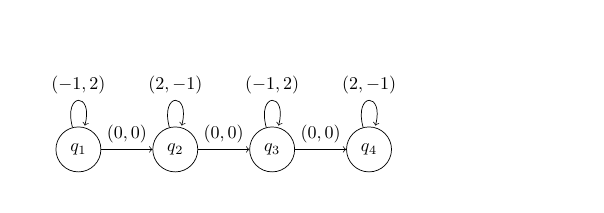
\begin{tikzpicture}[scale=0.25]
\usetikzlibrary{automata, positioning}
\scalebox{0.65}{
\node[state] (q1) {$q_1$};
\node[state, right=of q1] (q2) {$q_2$};
\node[state, right=of q2] (q3) {$q_3$};
\node[state, right=of q3] (q4) {$q_4$};

\path[->] (q1) edge [loop above] node[above] {$(-1,2)$} (q1) edge node[above] {$(0,0)$} (q2); 
\path[->] (q2) edge [loop above] node[above] {$(2,-1)$} (q2) edge node[above] {$(0,0)$} (q3);
\path[->] (q3) edge [loop above] node[above] {$(-1,2)$} (q3) edge node[above] {$(0,0)$} (q4);
\path[->] (q4) edge [loop above] node[above] {$(2,-1)$} (q4);
}
\end{tikzpicture}
\end{minipage}
\begin{minipage}{0.32\textwidth}
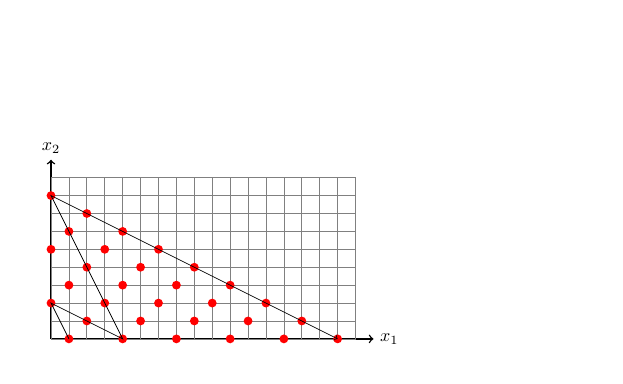
\begin{tikzpicture}[scale=0.35]
\scalebox{0.65}{
\draw[->, thick] (0, 0) -- (18, 0) node[right] {$x_1$};
\draw[->, thick] (0, 0) -- (0, 10) node[above] {$x_2$};

\draw[step=1, gray, thin] (0, 0) grid (17, 9);

\foreach \x in {1,4,7,10,13,16} \fill[red] (\x,0) circle (7pt);
\foreach \x in {2,5,8,11,14} \fill[red] (\x,1) circle (7pt);
\foreach \x in {0,3,6,9,12} \fill[red] (\x,2) circle (7pt);
\foreach \x in {1,4,7,10} \fill[red] (\x,3) circle (7pt);
\foreach \x in {2,5,8} \fill[red] (\x,4) circle (7pt);
\foreach \x in {0,3,6} \fill[red] (\x,5) circle (7pt);
\foreach \x in {1,4} \fill[red] (\x,6) circle (7pt);
\foreach \x in {2} \fill[red] (\x,7) circle (7pt);
\foreach \x in {0} \fill[red] (\x,8) circle (7pt);

\draw[->] (1,0) -- (0,2) -- (2,1) -- (4,0) -- (3,2) -- (2,4) -- (1,6) -- (0,8) -- (2,7) -- (4,6) -- (6,5) -- (8,4) -- (10,3) -- (12,2) -- (14,1) -- (16,0);
}
\end{tikzpicture}
\end{minipage}
\begin{minipage}{0.32\textwidth}
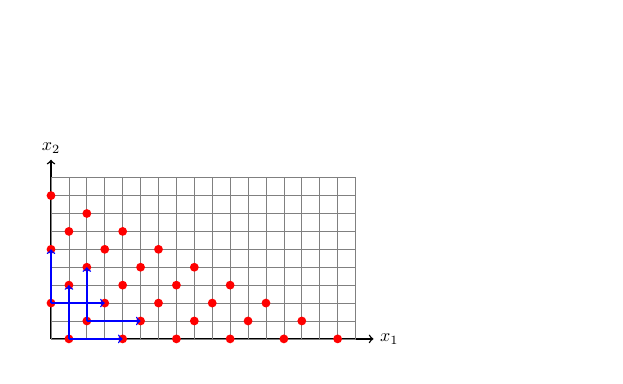
\begin{tikzpicture}[scale=0.35]
\scalebox{0.65}{
\draw[->, thick] (0, 0) -- (18, 0) node[right] {$x_1$};
\draw[->, thick] (0, 0) -- (0, 10) node[above] {$x_2$};

\draw[step=1, gray, thin] (0, 0) grid (17, 9);

\foreach \x in {1,4,7,10,13,16} \fill[red] (\x,0) circle (7pt);
\foreach \x in {2,5,8,11,14} \fill[red] (\x,1) circle (7pt);
\foreach \x in {0,3,6,9,12} \fill[red] (\x,2) circle (7pt);
\foreach \x in {1,4,7,10} \fill[red] (\x,3) circle (7pt);
\foreach \x in {2,5,8} \fill[red] (\x,4) circle (7pt);
\foreach \x in {0,3,6} \fill[red] (\x,5) circle (7pt);
\foreach \x in {1,4} \fill[red] (\x,6) circle (7pt);
\foreach \x in {2} \fill[red] (\x,7) circle (7pt);
\foreach \x in {0} \fill[red] (\x,8) circle (7pt);

\draw[->,blue,thick] (1,0) -- (4,0);
\draw[->,blue,thick] (1,0) -- (1,3);

\draw[->,blue,thick] (2,1) -- (5,1);
\draw[->,blue,thick] (2,1) -- (2,4);

\draw[->,blue,thick] (0,2) -- (3,2);
\draw[->,blue,thick] (0,2) -- (0,5);
}
\end{tikzpicture}
\end{minipage}
\caption{Left: 4-component \dvass $V_2$. 
Middle: the set $\reach_{q_4}(V_2, q_1(1,0))$ and a path $q_1(1,0) \tran q_4(16,0)$.
Right: bases 
%$A = \{(1,0),(2,1),(0,2)\}$ 
and periods 
%$P = \{(0,3),(3,0)\}$
 of an over-approximating semi-linear set $A+P^*$.}
\label{fig:zigzag}
\end{figure}

\begin{example}
For $k\geq 1$, let $V_k$ be a $(2k)$-component \dvass, where each component has just one state $q_i$
and one transition:
$(q_i, (-1,2), q_i)$ for odd $i$, and $(q_i, (2,-1), q_i)$ for even $i$.
Bridge transitions are $(q_i, (0,0), q_{i+1})$.
Figure~\ref{fig:zigzag} shows $V_2$ (left) and 
a path in $V_2$ from $s = q_1(1,0)$ to $t = q_4(16,0)$ together with 
the reachability set $\reach_{q_4}(V_2, s)$ (middle).
In general,
\begin{align} \label{eq:reachk}
X_k := \reach_{q_{2k}}(V_k, s) \ = \ \set{(x_1,x_2) \mid x_1+2x_2 \leq 4^k, \  x_1+2x_2 \equiv 1 \!\! \mod 3}.
\end{align}
Even if the size of the reachability set is 
exponential in $k$, for small $(x_1, x_2)$ it is periodic and the periods are small.
The set $X_k$ can be over-approximated by $A + P^*$ for $A = \set{(1,0),(2,1),(0,2)}$ and $P = \set{(0,3),(3,0)}$
(shown on the right of Figure~\ref{fig:zigzag}), namely for every $k\geq 1$ and $B\in\N$,
the set $X_k$ is \kanapka {$8$} {$B$}. 
For illustration, consider $Y := X_k \cap ((1,0) + P^*)$.
If $(1,0) + P^{\leq B} \subseteq X_k$ then $Y$ is a $B$-approximation
of $(1,0) + P^*$ with $\norm((1,0)), \norm(P) \leq 3 \leq 8$. 
Otherwise, there is some $(v_1, v_2) \in \big((1,0) + P^{\leq B}\big)\setminus X_k$, and
then $B$ is larger than $4^k$:
\[
%8B \geq 2(1 + 3B) \geq 2(v_1 + v_2) \geq v_1 + 2 v_2 > 
4^k < v_1 + 2 v_2 \leq 2(v_1 + v_2) \leq 2(1+3B) \leq 8B.
\]
Therefore by \eqref{eq:reachk}, each $(x_1,x_2) \in Y$ satisfies 
$\norm(x_1,x_2) = x_1 + x_2 \leq x_1 + 2x_2 \leq 4^k < 8B$, and thus
$Y$, seen as a union of singletons, is a union of 
linear sets with norm of base bounded by $8B$ and empty set of periods. 
In both cases, 
$Y$ is \kanapka {$8$} {$B$}. 
%The same intuition stays behind polynomial approximability of \dvass stated in Lemma~\ref{lem:2vass-sandwich}.
\end{example}


%%%%%%%%%%%%%%%%%%%%%%%%%%%%%%%%%%%%%%%%%%%%%%%%%%%%%%%%%%%%%%%%%%%%%%%%%%%%%%%%%%%%%%%%%%%%%%%%%%%%%%

%%%%%%%%%%%%%%%%%%%%%%%%%%%%%%%%%%%%%%%%%%%%%%
\begin{table*}[t]
\setlength{\tabcolsep}{3pt}
\centering
\renewcommand{\arraystretch}{1.1}
\tabcolsep=0.2cm
\begin{adjustbox}{max width=\textwidth}  % Set the maximum width to text width
\begin{tabular}{c| cccc ||  c| cc cc}
\toprule
General & \multicolumn{3}{c}{Preference} & Accuracy & Supervised & \multicolumn{3}{c}{Preference} & Accuracy \\ 
LLMs & PrefHit & PrefRecall & Reward & BLEU & Alignment & PrefHit & PrefRecall & Reward & BLEU \\ 
\midrule
GPT-J & 0.2572 & 0.6268 & 0.2410 & 0.0923 & Llama2-7B & 0.2029 & 0.803 & 0.0933 & 0.0947 \\
Pythia-2.8B & 0.3370 & 0.6449 & 0.1716 & 0.1355 & SFT & 0.2428 & 0.8125 & 0.1738 & 0.1364 \\
Qwen2-7B & 0.2790 & 0.8179 & 0.1593 & 0.2530 & Slic & 0.2464 & 0.6171 & 0.1700 & 0.1400 \\
Qwen2-57B & 0.3086 & 0.6481 & 0.6854 & 0.2568 & RRHF & 0.3297 & 0.8234 & 0.2263 & 0.1504 \\
Qwen2-72B & 0.3212 & 0.5555 & 0.6901 & 0.2286 & DPO-BT & 0.2500 & 0.8125 & 0.1728 & 0.1363 \\ 
StarCoder2-15B & 0.2464 & 0.6292 & 0.2962 & 0.1159 & DPO-PT & 0.2572 & 0.8067 & 0.1700 & 0.1348 \\
ChatGLM4-9B & 0.2246 & 0.6099 & 0.1686 & 0.1529 & PRO & 0.3025 & 0.6605 & 0.1802 & 0.1197 \\ 
Llama3-8B & 0.2826 & 0.6425 & 0.2458 & 0.1723 & \textbf{\shortname}* & \textbf{0.3659} & \textbf{0.8279} & \textbf{0.2301} & \textbf{0.1412} \\ 
\bottomrule
\end{tabular}
\end{adjustbox}
\caption{Main results on the StaCoCoQA. The left shows the performance of general LLMs, while the right presents the performance of the fine-tuned LLaMA2-7B across various strong benchmarks for preference alignment. Our method SeAdpra is highlighted in \textbf{bold}.}
\label{main}
\vspace{-0.2cm}
\end{table*}
%%%%%%%%%%%%%%%%%%%%%%%%%%%%%%%%%%%%%%%%%%%%%%%%%%%%%%%%%%%%%%%%%%%%%%%%%%%%%%%%%%%%%%%%%%%%%%%%%%%%
\begin{table}[h]
\centering
\renewcommand{\arraystretch}{1.02}
% \tabcolsep=0.1cm
\begin{adjustbox}{width=0.48\textwidth} % Adjust table width
\begin{tabularx}{0.495\textwidth}{p{1.2cm} p{0.7cm} p{0.95cm}p{0.95cm}p{0.7cm}p{0.7cm}}
     \toprule
    \multirow{2}{*}{\small \textbf{Dataset}} & \multirow{2}{*}{\small Model} & \multicolumn{2}{c}{\small Preference} & \multicolumn{2}{c}{\small Acc } \\ 
    & & \small \textit{PrefHit} & \small \textit{PrefRec} & \small \textit{Reward} & \small \textit{Rouge} \\ 
    \midrule
    \multirow{2}{*}{\small \textbf{Academia}}   & \small PRO & 33.78 & 59.56 & 69.94 & 9.84 \\ 
                                & \small \textbf{Ours} & 36.44 & 60.89 & 70.17 & 10.69 \\ 
    \midrule
    \multirow{2}{*}{\small \textbf{Chemistry}}  & \small PRO & 36.31 & 63.39 & 69.15 & 11.16 \\ 
                                & \small \textbf{Ours} & 38.69 & 64.68 & 69.31 & 12.27 \\ 
    \midrule
    \multirow{2}{*}{\small \textbf{Cooking}}    & \small PRO & 35.29 & 58.32 & 69.87 & 12.13 \\ 
                                & \small \textbf{Ours} & 38.50 & 60.01 & 69.93 & 13.73 \\ 
    \midrule
    \multirow{2}{*}{\small \textbf{Math}}       & \small PRO & 30.00 & 56.50 & 69.06 & 13.50 \\ 
                                & \small \textbf{Ours} & 32.00 & 58.54 & 69.21 & 14.45 \\ 
    \midrule
    \multirow{2}{*}{\small \textbf{Music}}      & \small PRO & 34.33 & 60.22 & 70.29 & 13.05 \\ 
                                & \small \textbf{Ours} & 37.00 & 60.61 & 70.84 & 13.82 \\ 
    \midrule
    \multirow{2}{*}{\small \textbf{Politics}}   & \small PRO & 41.77 & 66.10 & 69.52 & 9.31 \\ 
                                & \small \textbf{Ours} & 42.19 & 66.03 & 69.74 & 9.38 \\ 
    \midrule
    \multirow{2}{*}{\small \textbf{Code}} & \small PRO & 26.00 & 51.13 & 69.17 & 12.44 \\ 
                                & \small \textbf{Ours} & 27.00 & 51.77 & 69.46 & 13.33 \\ 
    \midrule
    \multirow{2}{*}{\small \textbf{Security}}   & \small PRO & 23.62 & 49.23 & 70.13 & 10.63 \\ 
                                & \small \textbf{Ours} & 25.20 & 49.24 & 70.92 & 10.98 \\ 
    \midrule
    \multirow{2}{*}{\small \textbf{Mean}}       & \small PRO & 32.64 & 58.05 & 69.64 & 11.51 \\ 
                                & \small \textbf{Ours} & \textbf{34.25} & \textbf{58.98} & \textbf{69.88} & \textbf{12.33} \\ 
    \bottomrule
\end{tabularx}
\end{adjustbox}
\caption{Main results (\%) on eight publicly available and popular CoQA datasets, comparing the strong list-wise benchmark PRO and \textbf{ours with bold}.}
\label{public}
\end{table}



%%%%%%%%%%%%%%%%%%%%%%%%%%%%%%%%%%%%%%%%%%%%%%%%%%%%%
\begin{table}[h]
\centering
\renewcommand{\arraystretch}{1.02}
\begin{tabularx}{0.48\textwidth}{p{1.45cm} p{0.56cm} p{0.6cm} p{0.6cm} p{0.50cm} p{0.45cm} X}
\toprule
\multirow{2}{*}{Method} & \multicolumn{3}{c}{Preference \((\uparrow)\)} & \multicolumn{3}{c}{Accuracy \((\uparrow)\)} \\ \cmidrule{2-4} \cmidrule{5-7}
& \small PrefHit & \small PrefRec & \small Reward & \small CoSim & \small BLEU & \small Rouge \\ \midrule
\small{SeAdpra} & \textbf{34.8} & \textbf{82.5} & \textbf{22.3} & \textbf{69.1} & \textbf{17.4} & \textbf{21.8} \\ 
\small{-w/o PerAl} & \underline{30.4} & 83.0 & 18.7 & 68.8 & \underline{12.6} & 21.0 \\
\small{-w/o PerCo} & 32.6 & 82.3 & \underline{24.2} & 69.3 & 16.4 & 21.0 \\
\small{-w/o \(\Delta_{Se}\)} & 31.2 & 82.8 & 18.6 & 68.3 & \underline{12.4} & 20.9 \\
\small{-w/o \(\Delta_{Po}\)} & \underline{29.4} & 82.2 & 22.1 & 69.0 & 16.6 & 21.4 \\
\small{\(PerCo_{Se}\)} & 30.9 & 83.5 & 15.6 & 67.6 & \underline{9.9} & 19.6 \\
\small{\(PerCo_{Po}\)} & \underline{30.3} & 82.7 & 20.5 & 68.9 & 14.4 & 20.1 \\ 
\bottomrule
\end{tabularx}
\caption{Ablation Results (\%). \(PerCo_{Se}\) or \(PerCo_{Po}\) only employs Single-APDF in Perceptual Comparison, replacing \(\Delta_{M}\) with \(\Delta_{Se}\) or \(\Delta_{Po}\). The bold represents the overall effect. The underlining highlights the most significant metric for each component's impact.}
\label{ablation}
% \vspace{-0.2cm}
\end{table}

\subsection{Dataset}

% These CoQA datasets contain questions and answers from the Stack Overflow data dump\footnote{https://archive.org/details/stackexchange}, intended for training preference models. 

Due to the additional challenges that programming QA presents for LLMs and the lack of high-quality, authentic multi-answer code preference datasets, we turned to StackExchange \footnote{https://archive.org/details/stackexchange}, a platform with forums that are accompanied by rich question-answering metadata. Based on this, we constructed a large-scale programming QA dataset in real-time (as of May 2024), called StaCoCoQA. It contains over 60,738 programming directories, as shown in Table~\ref{tab:stacocoqa_tags}, and 9,978,474 entries, with partial data statistics displayed in Figure~\ref{fig:dataset}. The data format of StaCoCoQA is presented in Table~\ref{fig::stacocoqa}.

The initial dataset \(D_I\) contains 24,101,803 entries, and is processed by the following steps:
(1) Select entries with "Questioner-picked answer" pairs to represent the preferences of the questioners, resulting in 12,260,106 entries in the \(D_Q\).
(2) Select data where the question includes at least one code block to focus on specific-domain programming QA, resulting in 9,978,474 entries in the dataset \(D_C\).
(3) All HTML tags were cleaned using BeautifulSoup \footnote{https://beautiful-soup-4.readthedocs.io/en/latest/} to ensure that the model is not affected by overly complex and meaningless content.
(4) Control the quality of the dataset by considering factors such as the time the question was posted, the size of the response pool, the difference between the highest and lowest votes within a pool, the votes for each response, the token-level length of the question and the answers, which yields varying sizes: 3K, 8K, 18K, 29K, and 64K. 
The controlled creation time variable and the data details after each processing step are shown in Table~\ref{tab:statistics}.

To further validate the effectiveness of SeAdpra, we also select eight popular topic CoQA datasets\footnote{https://huggingface.co/datasets/HuggingFaceH4/stack-exchange-preferences}, which have been filtered to meet specific criteria for preference models \cite{askell2021general}. Their detailed data information is provided in Table~\ref{domain}.
% Examples of some control variables are shown in Table~\ref{tab:statistics}.
% \noindent\textbf{Baselines}. 
% Following the DPO \cite{rafailov2024direct}, we evaluated several existing approaches aligned with human preference, including GPT-J \cite{gpt-j} and Pythia-2.8B \cite{biderman2023pythia}.  
% Next, we assessed StarCoder2 \cite{lozhkov2024starcoder}, which has demonstrated strong performance in code generation, alongside several general-purpose LLMs: Qwen2 \cite{qwen2}, ChatGLM4 \cite{wang2023cogvlm, glm2024chatglm} and LLaMA serials \cite{touvron2023llama,llama3modelcard}.
% Finally, we fine-tuned LLaMA2-7B on the StaCoCoQA and compared its performance with other strong baselines for supervised learning in preference alignment, including SFT, RRHF \cite{yuan2024rrhf}, Silc \cite{zhao2023slic}, DPO, and PRO \cite{song2024preference}.
%%%%%%%%%%%%%%%%%%%%%%%%%%%%%%%%%%%%%%%%%%%%%%%%%%%%%%%%%%%%%%%%%%%%%%%%%%%%%%%%%%%%%%%%%%%%%%%%%%%%%%%%%%%%%%%%%%%%%%%%%%%%%%%%%%

% For preference evaluation, traditional win-rate assessments are costly and not scalable. For instance, when an existing model \(M_A\) is evaluated against comparison methods \((M_B, M_C, M_D)\) in terms of win rates, upgrading model \(M_A\) would necessitate a reevaluation of its win rates against other models. Furthermore, if a new comparison method \(M_E\) is introduced, the win rates of model \(M_A\) against \(M_E\) would also need to be reassessed. Whether AI or humans are employed as evaluation mediators, binary preference between preferred and non-preferred choices or to score the inference results of the modified model, the costs of this process are substantial. 
% Therefore, from an economic perspective, we propose a novel list preference evaluation method. We utilize manually ranking results as the gold standard for assessing human preferences, to calculate the Hit and Recall, referred to as PrefHit and PrefRecall, respectively. Regardless of whether improving model \(M_A\) or expanding comparison method \(M_E\), only the calculation of PrefHit and PrefRecall for the modified model is required, eliminating the need for human evaluation. 
% We also employ a professional reward model\footnote{https://huggingface.co/OpenAssistant/reward-model-deberta-v3-large}
% for evaluation, denoted as the Reward metric.

% \subsection{Baseline} 
% Following the DPO \cite{rafailov2024direct}, we evaluated several existing approaches aligned with human preference, including GPT-J \cite{gpt-j} and Pythia-2.8B \cite{biderman2023pythia}.  
% Next, we assessed StarCoder2 \cite{lozhkov2024starcoder}, which has demonstrated strong performance in code generation, alongside several general-purpose LLMs: Qwen2 \cite{qwen2}, ChatGLM4 \cite{wang2023cogvlm, glm2024chatglm} and LLaMA serials \cite{touvron2023llama,llama3modelcard}.
% Finally, we fine-tuned LLaMA2-7B on the StaCoCoQA and compared its performance with other strong baselines for supervised learning in preference alignment, including SFT, RRHF \cite{yuan2024rrhf}, Silc \cite{zhao2023slic}, DPO, and PRO \cite{song2024preference}.
\subsection{Evaluation Metrics}
\label{sec: metric}
For preference evaluation, we design PrefHit and PrefRecall, adhering to the "CSTC" criterion outlined in Appendix \ref{sec::cstc}, which overcome the limitations of existing evaluation methods, as detailed in Appendix \ref{metric::mot}.
In addition, we demonstrate the effectiveness of thees new evaluation from two main aspects: 1) consistency with traditional metrics, and 2) applicability in different application scenarios in Appendix \ref{metric::ana}.
Following the previous \cite{song2024preference}, we also employ a professional reward.
% Following the previous \cite{song2024preference}, we also employ a professional reward model\footnote{https://huggingface.co/OpenAssistant/reward-model-deberta-v3-large} \cite{song2024preference}, denoted as the Reward.

For accuracy evaluation, we alternately employ BLEU \cite{papineni2002bleu}, RougeL \cite{lin2004rouge}, and CoSim. Similar to codebertscore \cite{zhou2023codebertscore}, CoSim not only focuses on the semantics of the code but also considers structural matching.
Additionally, the implementation details of SeAdpra are described in detail in the Appendix \ref{sec::imp}.
\subsection{Main Results}
We compared the performance of \shortname with general LLMs and strong preference alignment benchmarks on the StaCoCoQA dataset, as shown in Table~\ref{main}. Additionally, we compared SeAdpra with the strongly supervised alignment model PRO \cite{song2024preference} on eight publicly available CoQA datasets, as presented in Table~\ref{public} and Figure~\ref{fig::public}.

\textbf{Larger Model Parameters, Higher Preference.}
Firstly, the Qwen2 series has adopted DPO \cite{rafailov2024direct} in post-training, resulting in a significant enhancement in Reward.
In a horizontal comparison, the performance of Qwen2-7B and LLaMA2-7B in terms of PrefHit is comparable.
Gradually increasing the parameter size of Qwen2 \cite{qwen2} and LLaMA leads to higher PrefHit and Reward.
Additionally, general LLMs continue to demonstrate strong capabilities of programming understanding and generation preference datasets, contributing to high BLEU scores.
These findings indicate that increasing parameter size can significantly improve alignment.

\textbf{List-wise Ranking Outperforms Pair-wise Comparison.}
Intuitively, list-wise DPO-PT surpasses pair-wise DPO-{BT} on PrefHit. Other list-wise methods, such as RRHF, PRO, and our \shortname, also undoubtedly surpass the pair-wise Slic.

\textbf{Both Parameter Size and Alignment Strategies are Effective.}
Compared to other models, Pythia-2.8B achieved impressive results with significantly fewer parameters .
Effective alignment strategies can balance the performance differences brought by parameter size. For example, LLaMA2-7B with PRO achieves results close to Qwen2-57B in PrefHit. Moreover, LLaMA2-7B combined with our method SeAdpra has already far exceeded the PrefHit of Qwen2-57B.

\textbf{Rather not Higher Reward, Higher PrefHit.}
It is evident that Reward and PrefHit are not always positively correlated, indicating that models do not always accurately learn human preferences and cannot fully replace real human evaluation. Therefore, relying solely on a single public reward model is not sufficiently comprehensive when assessing preference alignment.

% In conclusion, during ensuring precise alignment, SeAdpra will focuse on PrefHit@1, even though the trade-off between PrefHit and PrefRecall is a common issue and increasing recall may sometimes lead to a decrease in hit rate. The positive correlation between Reward and BLEU, indicates that improving the quality of the generated text typically enhances the Reward. 
% Most importantly, evaluating preferences solely based on reward is clearly insufficient, as a high reward does not necessarily correspond to a high PrefHit or PrefRecall.
%%%%%%%%%%%%%%%%%%%%%%%%%%%%%%%%%%%%%%%%%%%
%%%%%%%%%%%%
\begin{figure}
  \centering
  \begin{subfigure}{0.49\linewidth}
    \includegraphics[width=\linewidth]{latex/pic/hit.png}
    \caption{The PrefHit}
    \label{scale:hit}
  \end{subfigure}
  \begin{subfigure}{0.49\linewidth}
    \includegraphics[width=\linewidth]{latex/pic/Recall.png}
    \caption{The PrefRecall}
    \label{scale:recall}
  \end{subfigure}
  \medskip
  \begin{subfigure}{0.48\linewidth}
    \includegraphics[width=\linewidth]{latex/pic/reward.png}
    \caption{The Reward}
    \label{scale:reward}
  \end{subfigure}
  \begin{subfigure}{0.48\linewidth}
    \includegraphics[width=\linewidth]{latex/pic/bleu.png}
    \caption{The BLEU}
    \label{scale:bleu}
  \end{subfigure}
  \caption{The performance with Confidence Interval (CI) of our SeAdpra and PRO at different data scales.}
  \label{fig:scale}
  % \vspace{-0.2cm}
\end{figure}
%%%%%%%%%%%%%%%%%%%%%%%%%%%%%%%%%%%%%%%%%%%%%%%%%%%%%%%%%%%%%%%%%%%%%%%%%%%%%%%%%%%%%%%%%%%%%%%%%%%%%%%%%%%%%%%%

\subsection{Ablation Study}

In this section, we discuss the effectiveness of each component of SeAdpra and its impact on various metrics. The results are presented in Table \ref{ablation}.

\textbf{Perceptual Comparison} aims to prevent the model from relying solely on linguistic probability ordering while neglecting the significance of APDF. Removing this Reward will significantly increase the margin, but PrefHit will decrease, which may hinder the model's ability to compare and learn the preference differences between responses.

\textbf{Perceptual Alignment} seeks to align with the optimal responses; removing it will lead to a significant decrease in PrefHit, while the Reward and accuracy metrics like CoSim will significantly increase, as it tends to favor preference over accuracy.

\textbf{Semantic Perceptual Distance} plays a crucial role in maintaining semantic accuracy in alignment learning. Removing it leads to a significant decrease in BLEU and Rouge. Since sacrificing accuracy recalls more possibilities, PrefHit decreases while PrefRecall increases. Moreover, eliminating both Semantic Perceptual Distance and Perceptual Alignment in \(PerCo_{Po}\) further increases PrefRecall, while the other metrics decline again, consistent with previous observations.


\textbf{Popularity Perceptual Distance} is most closely associated with PrefHit. Eliminating it causes PrefHit to drop to its lowest value, indicating that the popularity attribute is an extremely important factor in code communities.

% In summary, each module has a varying impact on preference and accuracy, but all outperform their respective foundation models and other baselines, as shown in Table \ref{main}, proving their effectiveness.


\subsection{Analysis and Discussion}

\textbf{SeAdpra adept at high-quality data rather than large-scale data.}
In StaCoCoQA, we tested PRO and SeAdpra across different data scales, and the results are shown in Figure~\ref{fig:scale}.
Since we rely on the popularity and clarity of questions and answers to filter data, a larger data scale often results in more pronounced deterioration in data quality. In Figure~\ref{scale:hit}, SeAdpra is highly sensitive to data quality in PrefHit, whereas PRO demonstrates improved performance with larger-scale data. Their performance on Prefrecall is consistent. In the native reward model of PRO, as depicted in Figure~\ref{scale:reward}, the reward fluctuations are minimal, while SeAdpra shows remarkable improvement.

\textbf{SeAdpra is relatively insensitive to ranking length.} 
We assessed SeAdpra's performance on different ranking lengths, as shown in Figure 6a. Unlike PRO, which varied with increasing ranking length, SeAdpra shows no significant differences across different lengths. There is a slight increase in performance on PrefHit and PrefRecall. Additionally, SeAdpra performs better at odd lengths compared to even lengths, which is an interesting phenomenon warranting further investigation.


\textbf{Balance Preference and Accuracy.} 
We analyzed the effect of control weights for Perceptual Comparisons in the optimization objective on preference and accuracy, with the findings presented in Figure~\ref{para:weight}.
When \( \alpha \) is greater than 0.05, the trends in PrefHit and BLEU are consistent, indicating that preference and accuracy can be optimized in tandem. However, when \( \alpha \) is 0.01, PrefHit is highest, but BLEU drops sharply.
Additionally, as \( \alpha \) changes, the variations in PrefHit and Reward, which are related to preference, are consistent with each other, reflecting their unified relationship in the optimization. Similarly, the variations in Recall and BLEU, which are related to accuracy, are also consistent, indicating a strong correlation between generation quality and comprehensiveness. 

%%%%%%%%%%%%%%%%%%%%%%%%%%%%%%%%%%%%%%%%%%%%%%%%%%%%%%%%%%%%%%%%%%%%%%%%%%%%%%%%%
\begin{figure}
  \centering
  \begin{subfigure}{0.475\linewidth}
    \includegraphics[width=\linewidth]{latex/pic/Rank1.png}
    \caption{Ranking length}
    \label{para:rank}
  \end{subfigure}
  \begin{subfigure}{0.475\linewidth}
    \includegraphics[width=\linewidth]{latex/pic/weights1.png}
    \caption{The \(\alpha\) in \(Loss\)}
    \label{para:weight}
  \end{subfigure}
  \caption{Parameters Analysis. Results of experiments on different ranking lengths and the weight \(\alpha\) in \(Loss\).}
  \label{fig:para}
  % \vspace{-0.2cm}
\end{figure}
%%%%%%%%%%%%%%%%%%%%%%%%%%%%%%%%%%%%%%%%%%%%
\begin{figure*}
  \centering
  \begin{subfigure}{0.305\linewidth}
    \includegraphics[width=\linewidth]{latex/pic/se2.pdf}
    \caption{The \(\Delta_{Se}\)}
    \label{visual:se}
  \end{subfigure}
  \begin{subfigure}{0.305\linewidth}
    \includegraphics[width=\linewidth]{latex/pic/po2.pdf}
    \caption{The \(\Delta_{Po}\)}
    \label{visual:po}
  \end{subfigure}
  \begin{subfigure}{0.305\linewidth}
    \includegraphics[width=\linewidth]{latex/pic/sv2.pdf}
    \caption{The \(\Delta_{M}\)}
    \label{visual:sv}
  \end{subfigure}
  \caption{The Visualization of Attribute-Perceptual Distance Factors (APDF) matrix of five responses. The blue represents the response with the highest APDF, and SeAdpra aligns with the fifth response corresponding to the maximum Multi-APDF in (c). The green represents the second response that is next best to the red one.}
  \label{visual}
  % \vspace{-0.2cm}
\end{figure*}
%%%%%%%%%%%%%%%%%%%%%%%%%%%%%%%%%%%%%%%%%
\textbf{Single-APDF Matrix Cannot Predict the Optimal Response.} We randomly selected a pair with a golden label and visualized its specific iteration in Figure~\ref{visual}.
It can be observed that the optimal response in a Single-APDF matrix is not necessarily the same as that in the Multi-APDF matrix.
Specifically, the optimal response in the Semantic Perceptual Factor matrix \(\Delta_{Se}\) is the fifth response in Figure~\ref{visual:se}, while in the Popularity Perceptual Factor matrix \(\Delta_{Po}\) (Figure~\ref{visual:po}), it is the third response. Ultimately, in the Multiple Perceptual Distance Factor matrix \(\Delta_{M}\), the third response is slightly inferior to the fifth response (0.037 vs. 0.038) in Figure~\ref{visual:sv}, and this result aligns with the golden label.
More key findings regarding the ADPF are described in Figure \ref{fig::hot1} and Figure \ref{fig::hot2}.

\putsec{related}{Related Work}

\noindent \textbf{Efficient Radiance Field Rendering.}
%
The introduction of Neural Radiance Fields (NeRF)~\cite{mil:sri20} has
generated significant interest in efficient 3D scene representation and
rendering for radiance fields.
%
Over the past years, there has been a large amount of research aimed at
accelerating NeRFs through algorithmic or software
optimizations~\cite{mul:eva22,fri:yu22,che:fun23,sun:sun22}, and the
development of hardware
accelerators~\cite{lee:cho23,li:li23,son:wen23,mub:kan23,fen:liu24}.
%
The state-of-the-art method, 3D Gaussian splatting~\cite{ker:kop23}, has
further fueled interest in accelerating radiance field
rendering~\cite{rad:ste24,lee:lee24,nie:stu24,lee:rho24,ham:mel24} as it
employs rasterization primitives that can be rendered much faster than NeRFs.
%
However, previous research focused on software graphics rendering on
programmable cores or building dedicated hardware accelerators. In contrast,
\name{} investigates the potential of efficient radiance field rendering while
utilizing fixed-function units in graphics hardware.
%
To our knowledge, this is the first work that assesses the performance
implications of rendering Gaussian-based radiance fields on the hardware
graphics pipeline with software and hardware optimizations.

%%%%%%%%%%%%%%%%%%%%%%%%%%%%%%%%%%%%%%%%%%%%%%%%%%%%%%%%%%%%%%%%%%%%%%%%%%
\myparagraph{Enhancing Graphics Rendering Hardware.}
%
The performance advantage of executing graphics rendering on either
programmable shader cores or fixed-function units varies depending on the
rendering methods and hardware designs.
%
Previous studies have explored the performance implication of graphics hardware
design by developing simulation infrastructures for graphics
workloads~\cite{bar:gon06,gub:aam19,tin:sax23,arn:par13}.
%
Additionally, several studies have aimed to improve the performance of
special-purpose hardware such as ray tracing units in graphics
hardware~\cite{cho:now23,liu:cha21} and proposed hardware accelerators for
graphics applications~\cite{lu:hua17,ram:gri09}.
%
In contrast to these works, which primarily evaluate traditional graphics
workloads, our work focuses on improving the performance of volume rendering
workloads, such as Gaussian splatting, which require blending a huge number of
fragments per pixel.

%%%%%%%%%%%%%%%%%%%%%%%%%%%%%%%%%%%%%%%%%%%%%%%%%%%%%%%%%%%%%%%%%%%%%%%%%%
%
In the context of multi-sample anti-aliasing, prior work proposed reducing the
amount of redundant shading by merging fragments from adjacent triangles in a
mesh at the quad granularity~\cite{fat:bou10}.
%
While both our work and quad-fragment merging (QFM)~\cite{fat:bou10} aim to
reduce operations by merging quads, our proposed technique differs from QFM in
many aspects.
%
Our method aims to blend \emph{overlapping primitives} along the depth
direction and applies to quads from any primitive. In contrast, QFM merges quad
fragments from small (e.g., pixel-sized) triangles that \emph{share} an edge
(i.e., \emph{connected}, \emph{non-overlapping} triangles).
%
As such, QFM is not applicable to the scenes consisting of a number of
unconnected transparent triangles, such as those in 3D Gaussian splatting.
%
In addition, our method computes the \emph{exact} color for each pixel by
offloading blending operations from ROPs to shader units, whereas QFM
\emph{approximates} pixel colors by using the color from one triangle when
multiple triangles are merged into a single quad.



\section{Conclusion and Future Work}\label{sec:con}
We proposed a novel bit-flip attack verification method, \tool, for QNNs, which is sound, complete, and arguably efficient. To achieve this, we introduced \symPoly, the first abstract domain tailored for networks with symbolic parameters. We implemented \tool as an end-to-end tool and conducted thorough experiments on various benchmarks with networks of different model sizes and quantization bit-widths, demonstrating its effectiveness and efficiency. 

While \symPoly may not represent the theoretically optimal abstract transformer for convex relaxations of weighted activation functions, it achieves optimal when restricting static abstractions to using only two linear constraints per neuron. 
Moreover, in terms of convex relaxation, the optimal abstraction transformer may not significantly enhance \symPoly, supported by the observation in~\cite{salman2019convex} that there is an inherent \emph{barrier} to tight relaxation-based verification methods. 
However, \tool could be integrated with complementary verification techniques, such as Branch-and-Bound for ReLU splitting~\cite{bunel2018unifiedviewpiecewiselinear} and optimizable lower bounds~\cite{xu2021fastcompleteenablingcomplete}, to improve the verification precision and scalability. We consider these promising extensions for future work.

\minor{Our verification approach targets bit-flip attacks on a single parameter. Extending such threat models to attack multiple parameters simultaneously, e.g., two out of $n$ parameters (i.e., $\mm=2$), would involve a straightforward modification of Algorithm~\ref{alg:overall} by traversing all $\binom{n}{2}=\frac{n\cdot(n-1)}{2}$ two-parameter combinations in the for-loop at line 3, leading to exponential computation growth. Hence, although the abstract domain \symPoly can handle multiple symbolic parameters simultaneously, how to efficiently and effectively partition all $\binom{\nn}{2}$ combinations into groups for abstraction-refinement poses a significant and non-trivial challenge, which is also a key focus in future work.}
  
% For further work, it would be interesting to investigate techniques for other network architectures, activation functions, and bit-flip attack settings, as well as to develop a more efficient verification method that does not require parameter traversal. This work represents a significant step towards these goals.

\section{Data-Availability Statement}
The source code of our tool and benchmarks are available at \cite{BFAVerifier}. %\url{https://anonymous.4open.science/r/BFAVerifier-B315}. 
%It will be submitted for Artifact Evaluation.

\begin{acks}
This study was supported by the 
Strategic Priority Research Program of CAS (Award ID: XDA0320101), 
the Ministry of Education, Singapore under its Academic Research Fund Tier 2 (T2EP20222-0037), and the Ministry of Education, Singapore under its Academic Research Fund Tier 3 (MOET32020-0003).	
% %CAS Project for Young Scientists in Basic Research (YSBR-040), 
% %ISCAS Fundamental Research Project (ISCAS-JCZD-202302),
% the Ministry of Education, Singapore under
% its Academic Research Fund Tier 3 (Award ID: MOET32020-0004), and the Ministry of Education, Singapore under its Academic Research Fund Tier 3 (Award ID:
% MOE-MOET32020-0003). 
Any opinions, findings, conclusions, or recommendations expressed in this material are those of the author(s) and do not reflect the views of the Ministry of Education, Singapore. 
\end{acks}


\bibliographystyle{ACM-Reference-Format}

\bibliography{yd-bibfile,ydbfa-bibfile}

% \newpage
\appendix



\section{Unexpected Questions}
\label{app:question}
Real-world questions do not always have the correct premises. For example, in the question "\begin{CJK}{UTF8}{gbsn}水俣病的传染途径是什么?\end{CJK}(What is the route of infection for Minamata disease?)", Minamata disease is not an infectious disease. Taking this situation into account, we add a small number of human-written questions with incorrect premises and LLM-generated questions with hard-to-verify premises in the question collection phase. The number of these questions in the total number of questions is about 3\%.

\section{Prompt for LLM Augmentation}
\label{app:aug}

\definecolor{titlecolor}{rgb}{0.9, 0.5, 0.1}
\definecolor{anscolor}{rgb}{0.2, 0.5, 0.8}
\definecolor{labelcolor}{HTML}{48a07e}
\begin{table*}[h]
	\centering
	
 % \vspace{-0.2cm}
	
	\begin{center}
		\begin{tikzpicture}[
				chatbox_inner/.style={rectangle, rounded corners, opacity=0, text opacity=1, font=\sffamily\scriptsize, text width=5in, text height=9pt, inner xsep=6pt, inner ysep=6pt},
				chatbox_prompt_inner/.style={chatbox_inner, align=flush left, xshift=0pt, text height=11pt},
				chatbox_user_inner/.style={chatbox_inner, align=flush left, xshift=0pt},
				chatbox_gpt_inner/.style={chatbox_inner, align=flush left, xshift=0pt},
				chatbox/.style={chatbox_inner, draw=black!25, fill=gray!7, opacity=1, text opacity=0},
				chatbox_prompt/.style={chatbox, align=flush left, fill=gray!1.5, draw=black!30, text height=10pt},
				chatbox_user/.style={chatbox, align=flush left},
				chatbox_gpt/.style={chatbox, align=flush left},
				chatbox2/.style={chatbox_gpt, fill=green!25},
				chatbox3/.style={chatbox_gpt, fill=red!20, draw=black!20},
				chatbox4/.style={chatbox_gpt, fill=yellow!30},
				labelbox/.style={rectangle, rounded corners, draw=black!50, font=\sffamily\scriptsize\bfseries, fill=gray!5, inner sep=3pt},
			]
											
			\node[chatbox_user] (q1) {
				\textbf{System prompt}
				\newline
				\newline
				You are a helpful and precise assistant for segmenting and labeling sentences. We would like to request your help on curating a dataset for entity-level hallucination detection.
				\newline \newline
                We will give you a machine generated biography and a list of checked facts about the biography. Each fact consists of a sentence and a label (True/False). Please do the following process. First, breaking down the biography into words. Second, by referring to the provided list of facts, merging some broken down words in the previous step to form meaningful entities. For example, ``strategic thinking'' should be one entity instead of two. Third, according to the labels in the list of facts, labeling each entity as True or False. Specifically, for facts that share a similar sentence structure (\eg, \textit{``He was born on Mach 9, 1941.''} (\texttt{True}) and \textit{``He was born in Ramos Mejia.''} (\texttt{False})), please first assign labels to entities that differ across atomic facts. For example, first labeling ``Mach 9, 1941'' (\texttt{True}) and ``Ramos Mejia'' (\texttt{False}) in the above case. For those entities that are the same across atomic facts (\eg, ``was born'') or are neutral (\eg, ``he,'' ``in,'' and ``on''), please label them as \texttt{True}. For the cases that there is no atomic fact that shares the same sentence structure, please identify the most informative entities in the sentence and label them with the same label as the atomic fact while treating the rest of the entities as \texttt{True}. In the end, output the entities and labels in the following format:
                \begin{itemize}[nosep]
                    \item Entity 1 (Label 1)
                    \item Entity 2 (Label 2)
                    \item ...
                    \item Entity N (Label N)
                \end{itemize}
                % \newline \newline
                Here are two examples:
                \newline\newline
                \textbf{[Example 1]}
                \newline
                [The start of the biography]
                \newline
                \textcolor{titlecolor}{Marianne McAndrew is an American actress and singer, born on November 21, 1942, in Cleveland, Ohio. She began her acting career in the late 1960s, appearing in various television shows and films.}
                \newline
                [The end of the biography]
                \newline \newline
                [The start of the list of checked facts]
                \newline
                \textcolor{anscolor}{[Marianne McAndrew is an American. (False); Marianne McAndrew is an actress. (True); Marianne McAndrew is a singer. (False); Marianne McAndrew was born on November 21, 1942. (False); Marianne McAndrew was born in Cleveland, Ohio. (False); She began her acting career in the late 1960s. (True); She has appeared in various television shows. (True); She has appeared in various films. (True)]}
                \newline
                [The end of the list of checked facts]
                \newline \newline
                [The start of the ideal output]
                \newline
                \textcolor{labelcolor}{[Marianne McAndrew (True); is (True); an (True); American (False); actress (True); and (True); singer (False); , (True); born (True); on (True); November 21, 1942 (False); , (True); in (True); Cleveland, Ohio (False); . (True); She (True); began (True); her (True); acting career (True); in (True); the late 1960s (True); , (True); appearing (True); in (True); various (True); television shows (True); and (True); films (True); . (True)]}
                \newline
                [The end of the ideal output]
				\newline \newline
                \textbf{[Example 2]}
                \newline
                [The start of the biography]
                \newline
                \textcolor{titlecolor}{Doug Sheehan is an American actor who was born on April 27, 1949, in Santa Monica, California. He is best known for his roles in soap operas, including his portrayal of Joe Kelly on ``General Hospital'' and Ben Gibson on ``Knots Landing.''}
                \newline
                [The end of the biography]
                \newline \newline
                [The start of the list of checked facts]
                \newline
                \textcolor{anscolor}{[Doug Sheehan is an American. (True); Doug Sheehan is an actor. (True); Doug Sheehan was born on April 27, 1949. (True); Doug Sheehan was born in Santa Monica, California. (False); He is best known for his roles in soap operas. (True); He portrayed Joe Kelly. (True); Joe Kelly was in General Hospital. (True); General Hospital is a soap opera. (True); He portrayed Ben Gibson. (True); Ben Gibson was in Knots Landing. (True); Knots Landing is a soap opera. (True)]}
                \newline
                [The end of the list of checked facts]
                \newline \newline
                [The start of the ideal output]
                \newline
                \textcolor{labelcolor}{[Doug Sheehan (True); is (True); an (True); American (True); actor (True); who (True); was born (True); on (True); April 27, 1949 (True); in (True); Santa Monica, California (False); . (True); He (True); is (True); best known (True); for (True); his roles in soap operas (True); , (True); including (True); in (True); his portrayal (True); of (True); Joe Kelly (True); on (True); ``General Hospital'' (True); and (True); Ben Gibson (True); on (True); ``Knots Landing.'' (True)]}
                \newline
                [The end of the ideal output]
				\newline \newline
				\textbf{User prompt}
				\newline
				\newline
				[The start of the biography]
				\newline
				\textcolor{magenta}{\texttt{\{BIOGRAPHY\}}}
				\newline
				[The ebd of the biography]
				\newline \newline
				[The start of the list of checked facts]
				\newline
				\textcolor{magenta}{\texttt{\{LIST OF CHECKED FACTS\}}}
				\newline
				[The end of the list of checked facts]
			};
			\node[chatbox_user_inner] (q1_text) at (q1) {
				\textbf{System prompt}
				\newline
				\newline
				You are a helpful and precise assistant for segmenting and labeling sentences. We would like to request your help on curating a dataset for entity-level hallucination detection.
				\newline \newline
                We will give you a machine generated biography and a list of checked facts about the biography. Each fact consists of a sentence and a label (True/False). Please do the following process. First, breaking down the biography into words. Second, by referring to the provided list of facts, merging some broken down words in the previous step to form meaningful entities. For example, ``strategic thinking'' should be one entity instead of two. Third, according to the labels in the list of facts, labeling each entity as True or False. Specifically, for facts that share a similar sentence structure (\eg, \textit{``He was born on Mach 9, 1941.''} (\texttt{True}) and \textit{``He was born in Ramos Mejia.''} (\texttt{False})), please first assign labels to entities that differ across atomic facts. For example, first labeling ``Mach 9, 1941'' (\texttt{True}) and ``Ramos Mejia'' (\texttt{False}) in the above case. For those entities that are the same across atomic facts (\eg, ``was born'') or are neutral (\eg, ``he,'' ``in,'' and ``on''), please label them as \texttt{True}. For the cases that there is no atomic fact that shares the same sentence structure, please identify the most informative entities in the sentence and label them with the same label as the atomic fact while treating the rest of the entities as \texttt{True}. In the end, output the entities and labels in the following format:
                \begin{itemize}[nosep]
                    \item Entity 1 (Label 1)
                    \item Entity 2 (Label 2)
                    \item ...
                    \item Entity N (Label N)
                \end{itemize}
                % \newline \newline
                Here are two examples:
                \newline\newline
                \textbf{[Example 1]}
                \newline
                [The start of the biography]
                \newline
                \textcolor{titlecolor}{Marianne McAndrew is an American actress and singer, born on November 21, 1942, in Cleveland, Ohio. She began her acting career in the late 1960s, appearing in various television shows and films.}
                \newline
                [The end of the biography]
                \newline \newline
                [The start of the list of checked facts]
                \newline
                \textcolor{anscolor}{[Marianne McAndrew is an American. (False); Marianne McAndrew is an actress. (True); Marianne McAndrew is a singer. (False); Marianne McAndrew was born on November 21, 1942. (False); Marianne McAndrew was born in Cleveland, Ohio. (False); She began her acting career in the late 1960s. (True); She has appeared in various television shows. (True); She has appeared in various films. (True)]}
                \newline
                [The end of the list of checked facts]
                \newline \newline
                [The start of the ideal output]
                \newline
                \textcolor{labelcolor}{[Marianne McAndrew (True); is (True); an (True); American (False); actress (True); and (True); singer (False); , (True); born (True); on (True); November 21, 1942 (False); , (True); in (True); Cleveland, Ohio (False); . (True); She (True); began (True); her (True); acting career (True); in (True); the late 1960s (True); , (True); appearing (True); in (True); various (True); television shows (True); and (True); films (True); . (True)]}
                \newline
                [The end of the ideal output]
				\newline \newline
                \textbf{[Example 2]}
                \newline
                [The start of the biography]
                \newline
                \textcolor{titlecolor}{Doug Sheehan is an American actor who was born on April 27, 1949, in Santa Monica, California. He is best known for his roles in soap operas, including his portrayal of Joe Kelly on ``General Hospital'' and Ben Gibson on ``Knots Landing.''}
                \newline
                [The end of the biography]
                \newline \newline
                [The start of the list of checked facts]
                \newline
                \textcolor{anscolor}{[Doug Sheehan is an American. (True); Doug Sheehan is an actor. (True); Doug Sheehan was born on April 27, 1949. (True); Doug Sheehan was born in Santa Monica, California. (False); He is best known for his roles in soap operas. (True); He portrayed Joe Kelly. (True); Joe Kelly was in General Hospital. (True); General Hospital is a soap opera. (True); He portrayed Ben Gibson. (True); Ben Gibson was in Knots Landing. (True); Knots Landing is a soap opera. (True)]}
                \newline
                [The end of the list of checked facts]
                \newline \newline
                [The start of the ideal output]
                \newline
                \textcolor{labelcolor}{[Doug Sheehan (True); is (True); an (True); American (True); actor (True); who (True); was born (True); on (True); April 27, 1949 (True); in (True); Santa Monica, California (False); . (True); He (True); is (True); best known (True); for (True); his roles in soap operas (True); , (True); including (True); in (True); his portrayal (True); of (True); Joe Kelly (True); on (True); ``General Hospital'' (True); and (True); Ben Gibson (True); on (True); ``Knots Landing.'' (True)]}
                \newline
                [The end of the ideal output]
				\newline \newline
				\textbf{User prompt}
				\newline
				\newline
				[The start of the biography]
				\newline
				\textcolor{magenta}{\texttt{\{BIOGRAPHY\}}}
				\newline
				[The ebd of the biography]
				\newline \newline
				[The start of the list of checked facts]
				\newline
				\textcolor{magenta}{\texttt{\{LIST OF CHECKED FACTS\}}}
				\newline
				[The end of the list of checked facts]
			};
		\end{tikzpicture}
        \caption{GPT-4o prompt for labeling hallucinated entities.}\label{tb:gpt-4-prompt}
	\end{center}
\vspace{-0cm}
\end{table*}
\begin{table*}

\centering

\begin{tabular}{|p{\textwidth}|}
\hline
\\ [2pt]
\par Here is a statement and a corresponding piece of reference text. Please complete the task as follows, strictly following the format I have given for the output:
\par (1) Find all the original key passages in the reference text that directly support the information in the statement (there may be more than one, find each one). Output one original key passage per line and the information in the statement it directly supports in the format “Key passage {number}: {key passage} (information in the supporting statement: {supporting information})”.
\par (2) Please group key passages, each group contains key passages supporting the same or related information in the statement, output one line of the grouping results in the format of “Key passage grouping: Group 1: (first group of key passage numbers), Group 2: (second group of key passage numbers) ...”. For example, if there are 2 pieces of information in the statement, key paragraph 1 supports information 1, key paragraph 2 supports information 2, and key paragraph 3 supports information 1, then the output is “Key Paragraph Grouping: Group 1: (1, 3), Group 2: (2)”.
\par (3) Select a group of key text segments and modify the parts of them that support the information in the statement to meet the following requirements:
\par - The modification should make it impossible for the key passage to fully support the corresponding information in the statement.
\par - The modifications should maintain the logical flow of the key passages and no contradictions between the information in the key passages.
\par - The modification should keep the key paragraph logically coherent in the context of the reference text and not contradict the rest of the reference text.
\par - Modify only the parts that support the information in a statement, leaving the rest unchanged.
\par - If there is more than one key passage in a set, the information in them should remain consistent after revision.
\par You need to try two methods of modification:
\par - Changing the message: modifying the message in one part of the key paragraph to another. Do not make changes that directly conflict with the original information. For example, if the original message is “The Audi A7 Signature Edition has a faster top speed than its predecessor”, an appropriate change would be “The Audi A7 Luxury Edition has a faster top speed than its predecessor”, and an inappropriate change1 would be “The Audi A7 Signature Edition has a slower top speed than its predecessor” (using an antonym, which is in direct conflict with the original message), and inappropriate modification 2 is ‘The top speed of the Audi A7 Signature Edition is not faster than the previous generation’ (adding a negative word, which is in direct conflict with the original message).
\par - Delete Information: Remove information from a place in a key paragraph. If the key paragraph is a complete sentence, it should still be a complete sentence after deleting the information. For example, if the original paragraph reads “Due to weather conditions, the project was delayed until March 15” (complete sentence), an appropriate change would be “Due to weather conditions, the project was delayed until March” (still a complete sentence), an inappropriate change would be “Due to the weather” (no longer a complete sentence).
\par For each method, output the key passage that was modified and check its logical fluency, giving an integer within 1 to 10 as a rating (higher means more fluent). Output one modified key passage per line in the format “{method}-modified key passage {number}: {modified key passage} (logical fluency: {score})”.
\\ [5pt]
\\ [5pt]
\hline

\end{tabular}

\caption{\label{tab:prompt_en} The complete prompt for the LLM augmentation (translated into English).}
\end{table*}

See Table~\ref{tab:prompt} for the prompt for LLM augmentation. Table~\ref{tab:prompt_en} provides an English version.

\section{Instructions for Annotators}
\label{app:ann}
\subsection{First Stage}
In the first stage, we provide the annotators with the question, answer, statement, and cited documents. What LLM considers to be key segments are highlighted in red in the cited documents (see Figure~\ref{fig:stage} for an example). We instruct the annotators to follow the process below:

\par (1) First look at the highlighted text. If the highlighted text fully supports the statement, then the annotation is positive; if the highlighted text contradicts the statement, then the annotation is negative.

\par (2) If the annotation cannot be derived from the highlighted text, then look at the rest of the documents to make the annotation. When the documents fully support the statement, the label is positive, and when there is any information in the statement that contradicts the documents or information that is not mentioned in the documents, the label is negative.

\subsection{Second Stage}

In the second stage, we provide the annotator with the statement and the modified documents. In the documents, the modified parts are highlighted in green, where the dashed and crossed-out text is deleted and the rest is added (see Figure~\ref{fig:stage} for examples). 

For the annotation of whether the quality of the modification is acceptable, the annotators are instructed to note that qualified modifications need to satisfy the following two requirements: (1) There are no contradictions within each modified document. (2) The modified key segments are fluent in their own right and in the context of the document. The annotation for support is the same as the first stage, but based on the modified documents.

 
\section{Input and Training Details}
\label{app:detail}
We input the statement and the cited documents into the model and ask the model to determine whether the statement is fully supported by the documents, outputting yes or no. For input, we label and concatenate the cited documents in order (as shown in Table~\ref{tab:dataset}). For training, we use the following settings: For training, we use the following settings: learning rate is 5e-4, number of epochs is 10, scheduler is cosine scheduler, warmup ratio is 0.03, batch size is 256, and LoRA setting is $r=8$, $a=32$ and 0.1 dropout. We report the model performance for the epoch that achieves the best performance on the dev set.
\label{app:detail}



\section{Related Works}
Language models are known to produce hallucinations - statements that are inaccurate or unfounded~\citep{MaynezNBM20,HuCLGWYG24}. To address this limitation, recent research has focused on augmenting LLMs with external tools such as retrievers~\citep{GuuLTPC20,BorgeaudMHCRM0L22,LiuCtrla2024} and search engines~\citep{WebGPT2021, Komeili0W22, TanGSXLFLWSLS24}. While this approach suggests that generated content is supported by external references, the reliability of such attribution requires careful examination. Recent studies have investigated the validity of these attributions. \citet{DBLP:conf/emnlp/LiuZL23} conducted human evaluations to assess the verifiability of responses from generative search engines. \citet{hu2024evaluate} further investigate the reliability of such attributions when giving adversarial questions to RAG systems. Their findings revealed frequent occurrences of unsupported statements and inaccurate citations, highlighting the need for rigorous attribution verification~\citep{RashkinNLA00PTT23}. However, human evaluation processes are resource-intensive and time-consuming. To overcome these limitations, existing efforts~\citep{GaoDPCCFZLLJG23,DBLP:conf/emnlp/GaoYYC23} proposed an automated approach using Natural Language Inference models to evaluate attribution accuracy. While several English-language benchmarks have been developed for this purpose~\citep{DBLP:conf/emnlp/YueWCZS023}, comparable resources in Chinese are notably lacking. Creating such datasets presents unique challenges, particularly in generating realistic negative samples (unsupported citations).  To address this gap, we introduce the first large-scale Chinese dataset for citation faithfulness detection, developed through a cost-effective two-stage manual annotation process.

\begin{figure*}
    \centering
    \includegraphics[width=0.3\textwidth]{appendix/s1.png}
    \includegraphics[width=0.3\textwidth]{appendix/s2-m.png}
    \includegraphics[width=0.3\textwidth]{appendix/s2-d.png}
    \caption{Examples of interfaces that provide samples to the annotators. The first figure shows an example of the first stage. The last two images show the second stage with the same sample modified (information changed/deleted).}
    \label{fig:stage}
\end{figure*}



\end{document}
